\section{Robot (Imitation) Learning}
\label{sec:learning-bc-single}

\epigraph{\emph{The best material model for a cat is another, or preferably the same cat}}{Norbert Wiener}

\begin{tldr}
Behavioral Cloning provides a natural platform to learn from real-world interactions without the need to design any reward function, and generative models prove more effective than point-wise policies at dealing with multimodal demonstration datasets.
\end{tldr}

\begin{figure}
    \centering
    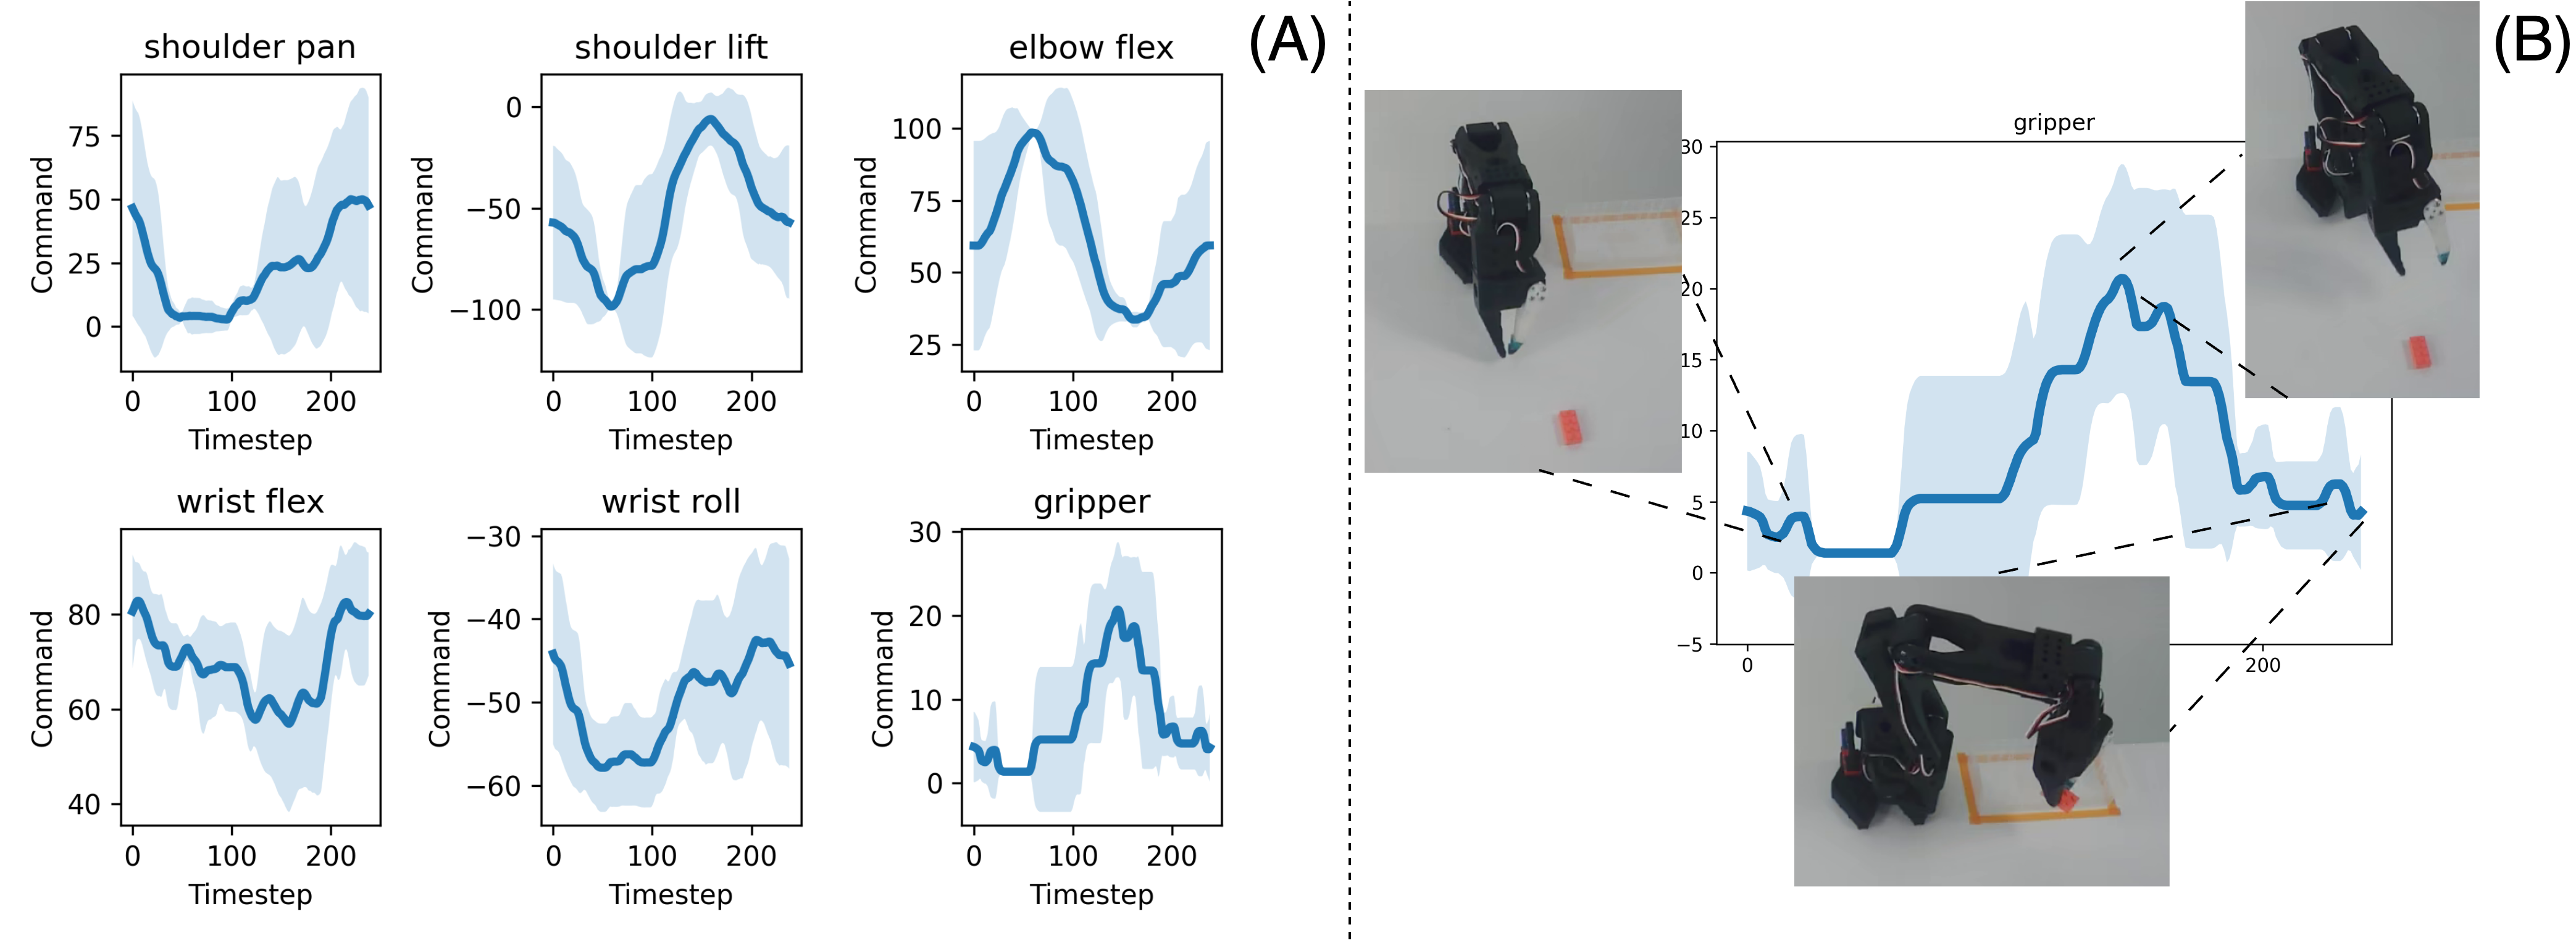
\includegraphics[width=0.8\textwidth]{figures/ch4/ch4-bc-trajectories.png}
    \caption{(A) Average (with standard deviation) evolution of the actuation levels over the first 5 recorded episodes in \url{lerobot/svla_so101_pickplace}. Proprioperceptive state provide invaluable to determine the robot's state during an episode. (B) Camera frames are also recorded alongside measurements on the robot's state, capturing information about the robot's interaction with its environment.}
    \label{fig:ch4-bc-trajectories}
\end{figure}

Learning from human demonstrations provides a pragmatic alternative to the reinforcement-learning pipeline discussed in Section~\ref{sec:learning-rl}.
Indeed, in real-world robotics online exploration is typically \highlight{costly and potentially unsafe}, and designing (dense) reward signals is a \highlight{brittle and task-specific} process.
In general, success detection itself may often require bespoke instrumentation, while episodic training demands reliable resets---all factors complicating training RL algorithms on hardware at scale.
Behavioral Cloning (BC) sidesteps these constraints by casting control an imitation learning problem, leveraging previously collected expert demonstrations.
Most notably, by learning to imitate autonomous systems naturally adhere to the objectives, preferences, and success criteria implicitly encoded in the data, which obviates reduces early-stage exploratory failures and obviates hand-crafted reward shaping altogether.

Formally, let \( \mathcal D = \{ \tau^{(i)} \}_{i=1}^N \) be a set of expert trajectories, with \( \tau^{(i)} = \{(o_t^{(i)}, a_t^{(i)})\}_{t=0}^{T_i} \) representing the \(i\)-th trajectory in \( \mathcal D \), \(o_t \in \obsspace \) denoting observations (e.g., images and proprioception altogether), and \(a_t \in \actionspace \) the expert actions.
Typically, observations \( o \in \obsspace \) consist of both image and proprioperceptive information, while actions \( a \in \actionspace \) represent control specifications for the robot to execute, e.g. a joint configuration.
Note that differently from Section~\ref{sec:learning-rl}, in the imitation learning context \( \mathcal D \) denotes an offline dataset collecting \( N \) length-\( T_i \) reward-free (expert) human trajectories \( \tau^{(i)} \), and \emph{not} the environment dynamics.
Similarily, in this section \( \tau^{(i)} \) represent a length-\(T_i\) trajectory of observation-action pairs, which crucially \emph{omits entirely any reward} information.
Figure~\ref{fig:ch4-bc-trajectories} graphically shows trajectories in terms of the average evolution of the actuation on the 6 joints over a group of teleoperated episodes for the SO-100 manipulator.
Notice how proprioperceptive states are captured jointly with camera frames over the course of the recorded episodes, providing a unified high-frame rate collection of teleoperation data.
Figure~\ref{fig:ch4-observation-action-mapping} shows \( (o_t, a_t) \)-pairs for the same dataset, with the actions performed by the human expert illustrated just alongside the corresponding observation.
In principle, (expert) trajectories \( \tau^{(i)} \) can have different lengths since demonstrations might exhibit multi-modal strategies to attain the same goal, resulting in possibly multiple, different behaviors.

% NOTE(fracapuano): maybe change RL notation to T for transitions and eta for trajectories to avoid specifying difference of notation in here?
\begin{figure}
    \centering
    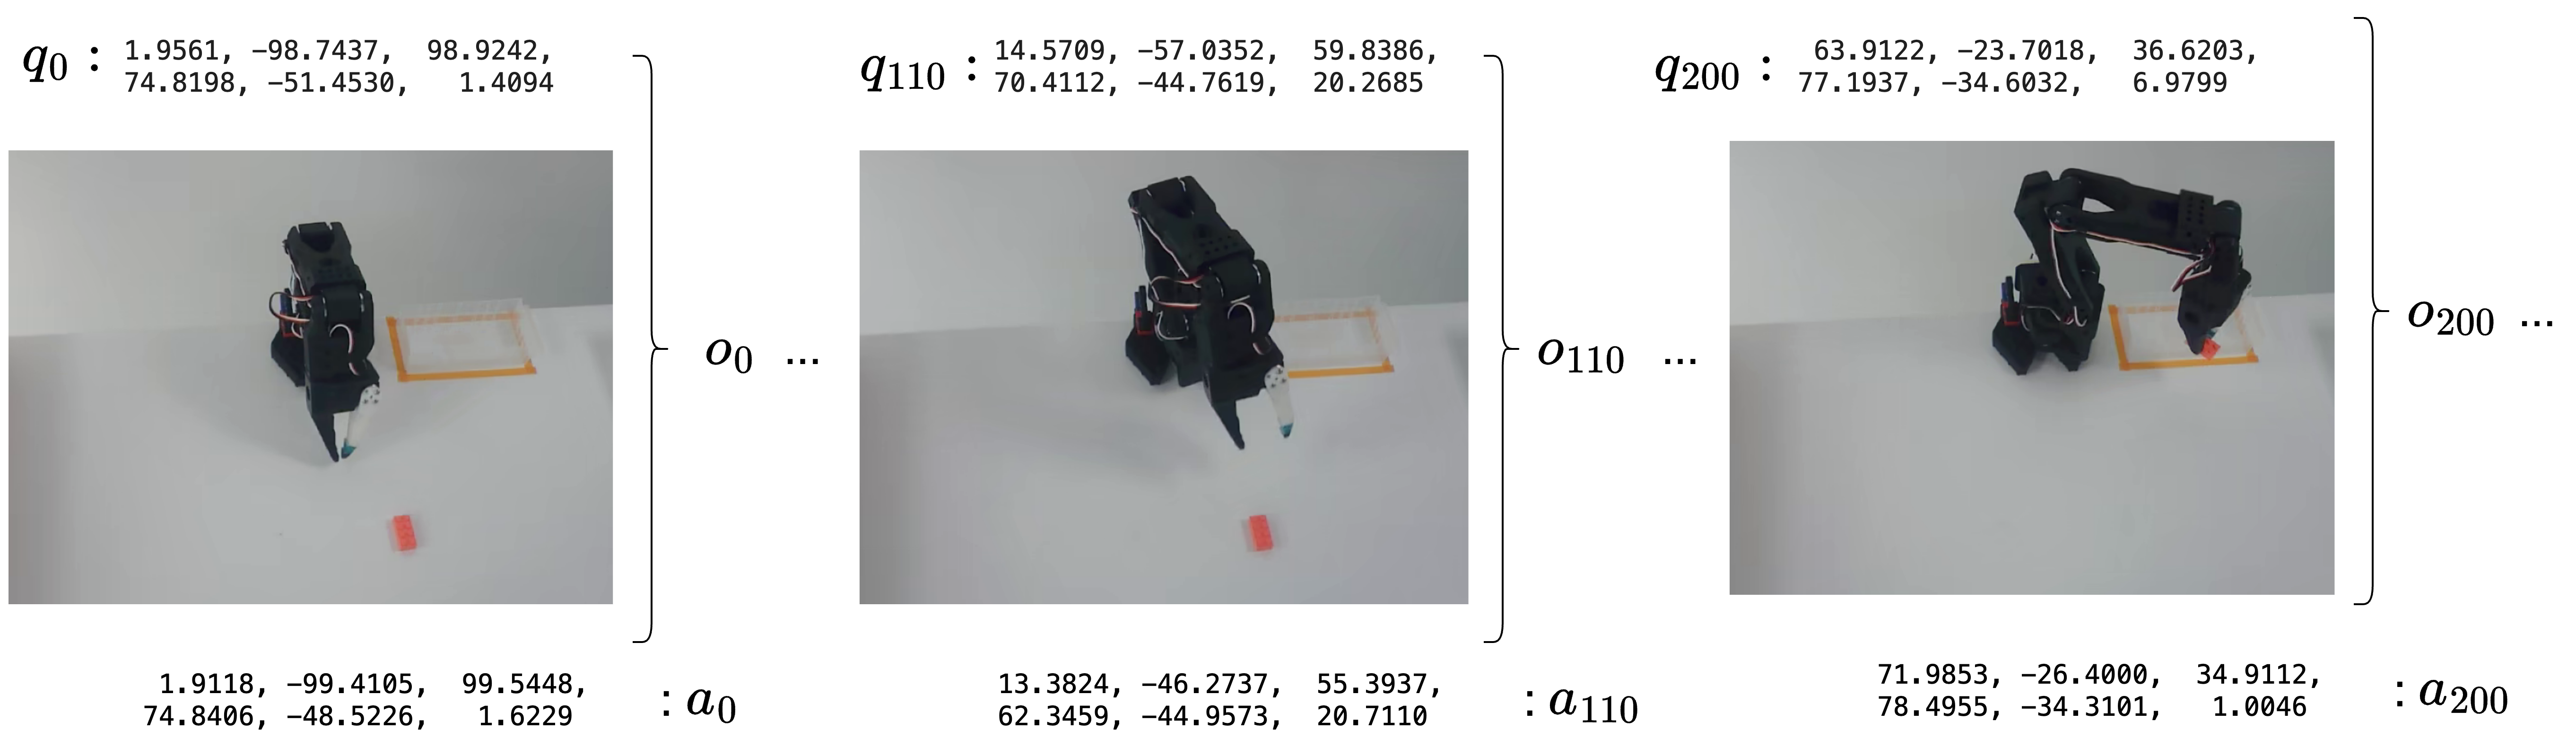
\includegraphics[width=0.9\textwidth]{figures/ch4/ch4-observation-action-mapping.png}
    \caption{Sample observations and action pairs over the course of a given trajectory recorded in \url{lerobot/svla_so101_pickplace}. Observations, comprising of both proprioperceptive and visual information, are recorded alongside the configuration of a second, leader robot controlled by a human expert, providing complete information for regressing actions given observation.}
    \label{fig:ch4-observation-action-mapping}
\end{figure}

Behavioral Cloning (BC)~\citep{pomerleauALVINNAutonomousLand1988a} aims at synthetizing synthetic behaviors by learning the mapping from observations to actions, and in its most natural formulation can be effectively tackled as a \emph{supevised} learning problem, consisting of learning the (deterministic) mapping \(f: \obsspace \mapsto \actionspace, \ a_t = f(o_t) \) by solving
\begin{equation}\label{eq:loss-minimization-SL}
    \min_{f} \mathbb{E}_{(o_t, a_t) \sim p(\bullet)} \mathcal L(a_t, f(o_t)),
\end{equation}
for a given risk function \( \mathcal L:  \mathcal A \times \mathcal A \mapsto \mathbb{R}, \ \mathcal L (a, a^\prime) \).

Typically, the expert's joint observation-action distribution \( p: \obsspace \times \actionspace \mapsto [0,1] \) such that \( (o,a) \sim p(\bullet) \) is assumed to be unknown, in keeping with a classic Supervised Learning (SL) framework\footnote{Throughout, we will adopt the terminology and notation for SL introduced in~\citet{shalev-shwartzUnderstandingMachineLearning2014}}.
However, differently from standard SL's assumptions, the samples collected in \( \mathcal D \), correspoding to observations of the underlying \( p \) are \emph{not} i.i.d., as expert demonstrations are collected \emph{sequentially} in trajectories.
In practice, this aspect can be partially mitigated by considering pairs in a non-sequential order---\emph{shuffling} the samples in \(\mathcal D \)---so that the expected risk under \( p \) can be approximated using MC estimates, although estimates may in general be less accurate.
Another strategy to mitigate the impact of regressing over non-i.i.d. samples relies on the possibility of interleaving BC and data collection~\citep{rossReductionImitationLearning2011}, aggregating multiple datasets iteratively.
However, because we only consider the case where a single offline dataset \( \mathcal D \) of (expert) trajectories is already available, dataset aggregation falls out of scope.

Despite the inherent challenges of learning on non-i.i.d. data, the BC formulation affords several operational advantages in robotics.
First, training happens offline and typically uses expert human demonstration data, hereby severily limiting exploration risks by preventing the robot from performing dangerous actions altogether.
Second, reward design is entirely unnecessary in BC, as demonstrations already reflect human intent and task completion.
This also mitigates the risk of misalignment and specification gaming (\emph{reward hacking}), otherwise inherent in purely reward-based RL~\citep{heessEmergenceLocomotionBehaviours2017}.
Third, because expert trajectories encode terminal conditions, success detection and resets are implicit in the dataset.
Finally, BC scales naturally with growing corpora of demonstrations collected across tasks, embodiments, and environments.
However, BC can in principle only learn behaviors that are, at most, as good as the one exhibited by the demonstrator, and thus critically provides no mitigation for the suboptimal decision making that might be enaced by humans.
Still, while problematic in sequential-decision making problems for which expert demonstrations are not generally available---data migth be expensive to collect, or human performance may be inherently suboptimal---many robotics applications benefit from relative cheap pipelines to acquire high-quality trajectories generated by humans, thus justifying BC approaches.

\begin{figure}
    \centering
    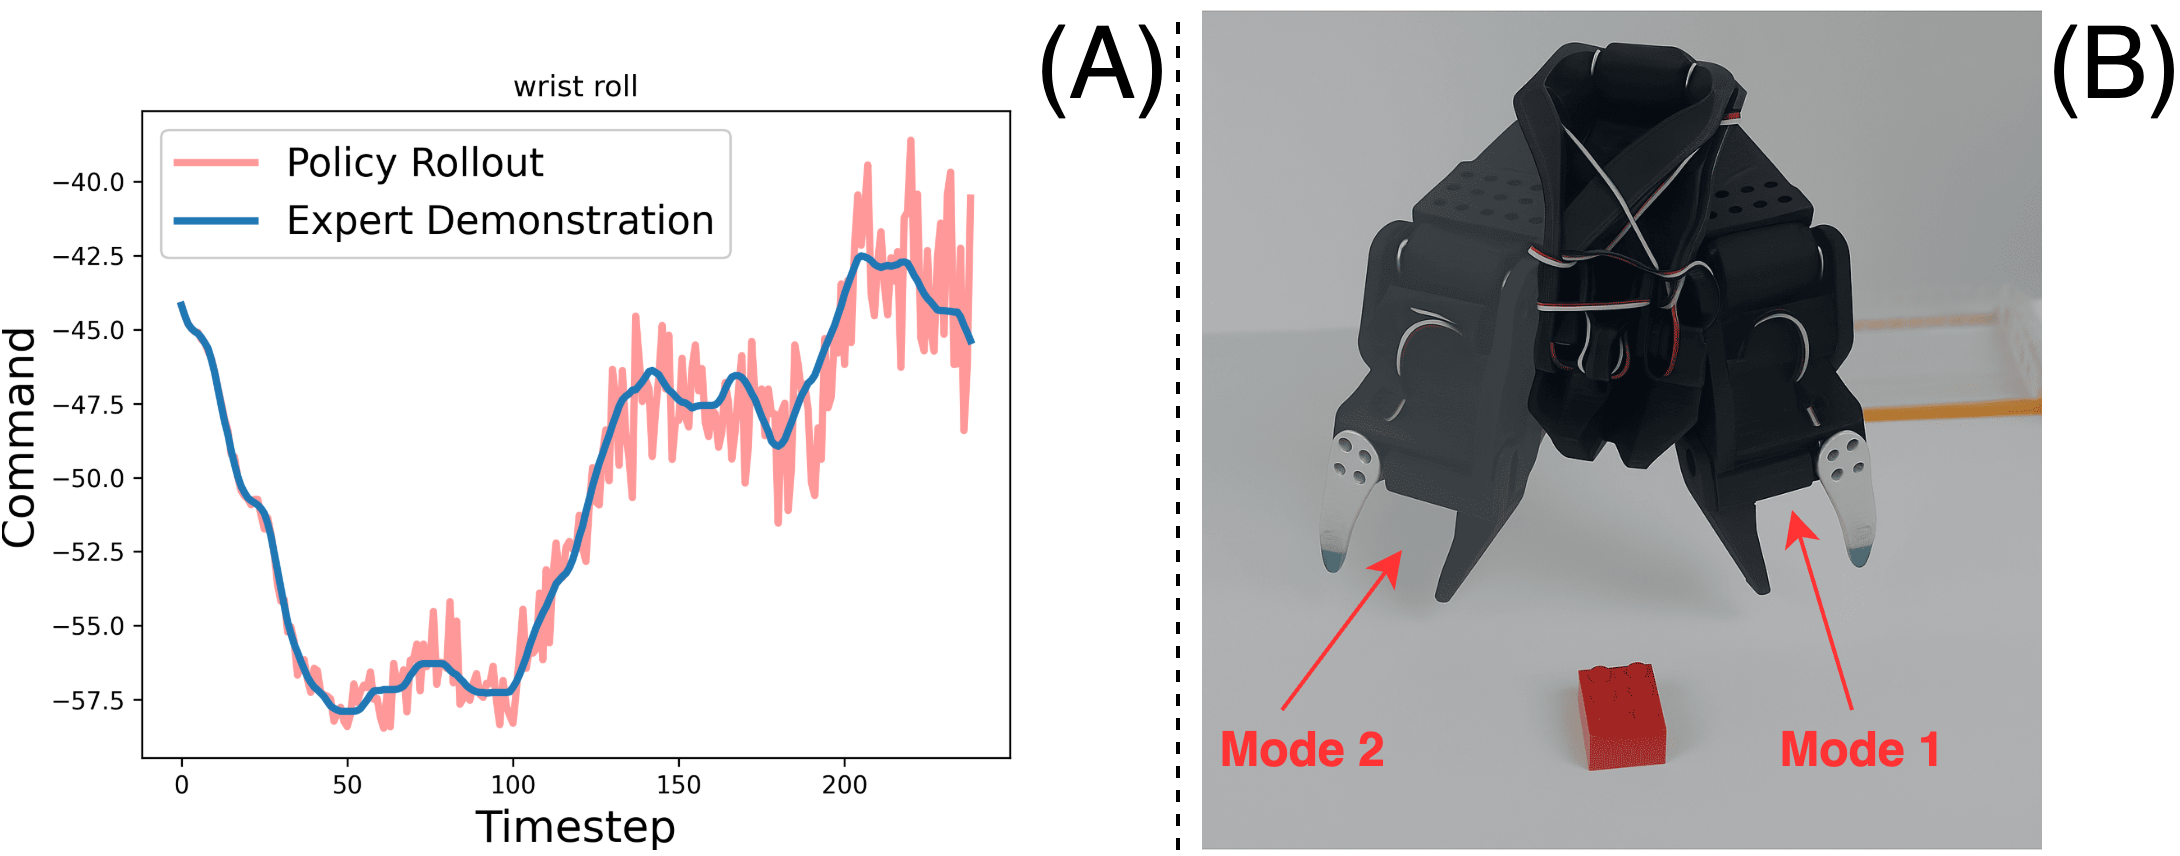
\includegraphics[width=0.8\textwidth]{figures/ch4/ch4-issues-with-bc.png}
    \caption{Point-wise policies suffer from limitations due to (A) covariate shifts and poor approximation of (B) multimodal demonstrations. (A) Initially small errors may drive the policy out of distribution, incuring in a vicious circle ultimately resulting in failure. (B) Both modes of reaching for a target object in a scene, either left or right-first, are equally as good and thus equally as likely to be present in a dataset of human demonstrations, ultimately resulting in multimodal demonstrations.}
    \label{fig:ch4-issues-with-bc}
\end{figure}

While conceptually elegant, point-estimate policies \( f : \obsspace \mapsto \actionspace \) learned by solving \ref{eq:loss-minimization-SL} have been observed to suffer from (1) compounding errors~\citep{rossReductionImitationLearning2011} and (2) poor fit to multimodal distributions~\citep{florenceImplicitBehavioralCloning2022, keGraspingChopsticksCombating2020}.
Figure~\ref{fig:ch4-issues-with-bc} illustrates these two key issues related to learning \emph{explicit policies}~\citep{florenceImplicitBehavioralCloning2022}.
Besides sequentiality in \( \mathcal D \), compounding errors due to \emph{covariate shift} may also prove catastrophic, as even small \( \epsilon \)-prediction errors \( 0 < \Vert \mu(o_t) - a_t \Vert \leq \epsilon \) can quickly drive the policy into out-of-distribution states, incuring in less confident generations and thus errors compounding (Figure~\ref{fig:ch4-issues-with-bc}, left).Moreover, point-estimate policies typically fail to learn \emph{multimodal} targets, which are very common in human demonstrations solving robotics problems, since multiple trajectories can be equally as good towards the accomplishment of a goal (e.g., symmetric grasps, Figure~\ref{fig:ch4-issues-with-bc}, right).
In particular, unimodal regressors tend to average across modes, yielding indecisive or even unsafe commands~\citep{florenceImplicitBehavioralCloning2022}.
To address poor multimodal fitting,~\citet{florenceImplicitBehavioralCloning2022} propose learning the generative model \( p(o, a) \) underlying the samples in \( \mathcal D \), rather than an explicitly learning a prediction function \( f(o) = a \).

\subsection{A (Concise) Introduction to Generative Models}
% Generative Modeling
Generative Models (GMs) aim to learn the stochastic process underlying the very generation of the data collected, and typically do so by fitting a probability distribution that approximates the unknown \emph{data distribution}, \( p \).
In the case of BC, this unknown data distribution \( p \) represents the expert's joint distribution over \( (o, a) \)-pairs.
Thus, given a finite set of \( N \) pairs \(\mathcal D = \{ (o,a)_i \}_{i=0}^N\) used as an imitation learning target (and thus assumed to be i.i.d.), GM seeks to learn a \emph{parametric} distribution \( p_\theta(o,a) \) such that (1) new samples \( (o,a) \sim p_\theta(\bullet) \) resemble those stored in \( \mathcal D \), and (2) high likelihood is assigned to the observed regions of the unobservable \( p \).
Likelihood-based learning provides a principled training objective to achieve both objectives, and it is thus extensively used in GM~\citep{prince2023understanding}.

% VAEs
\paragraph{Variational Auto-Encoders}

\begin{figure}
    \centering
    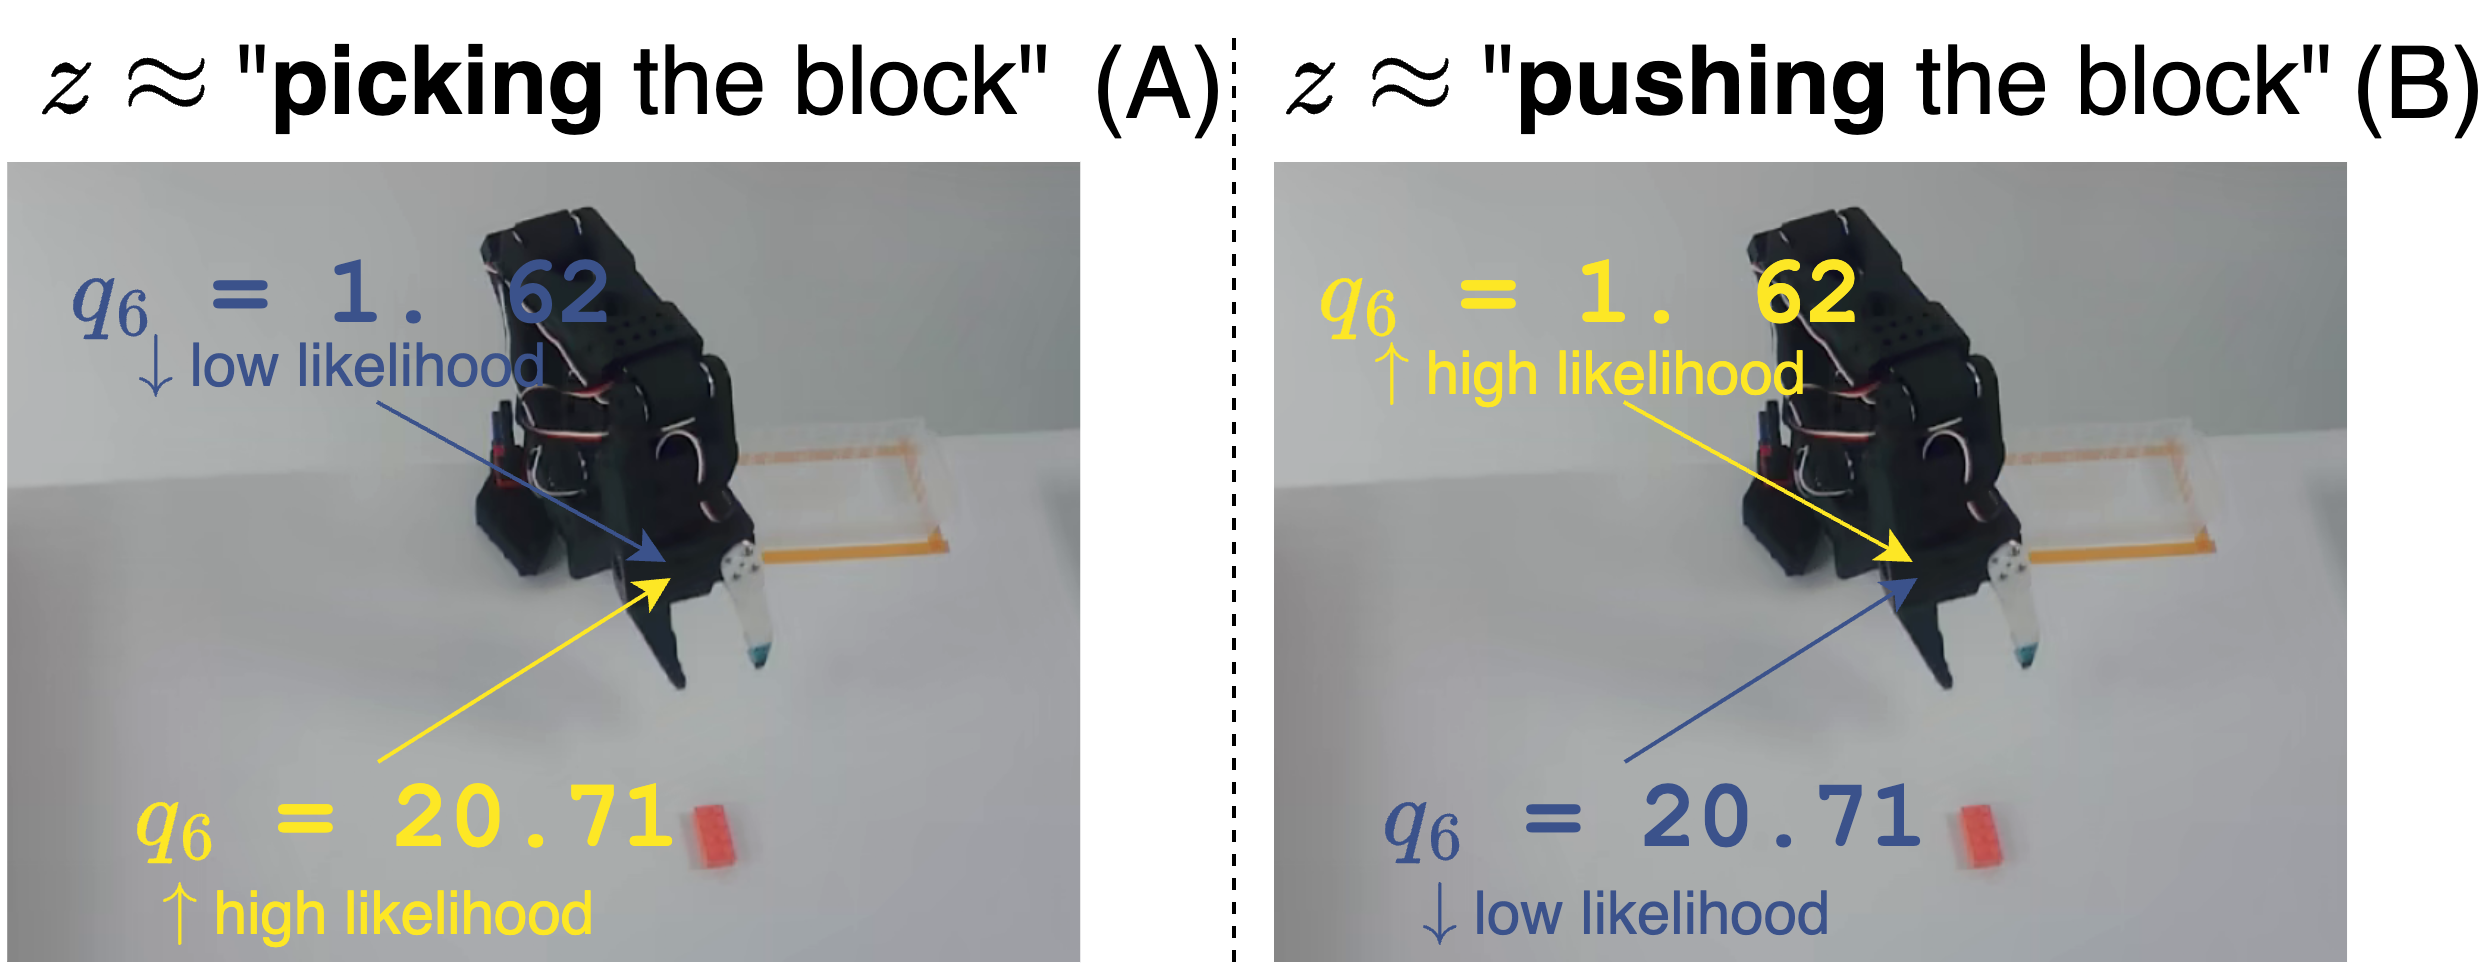
\includegraphics[width=0.8\textwidth]{figures/ch4/ch4-task-effect-on-pairs.png}
    \caption{Intuitively, latent variable in a single latent model may contain information regarding the task being performed, which directly results in the likelihood of the same observation-action pair being different for two different tasks. When (A) picking a block the likelihood of a wide gripper's opening should be higher than narrower one, while it should be the opposite when (B) pushing the block.}
    \label{fig:ch4-task-effect-on-pairs}
\end{figure}

A common inductive bias used in GM posits samples \( (o,a) \) are influenced from an unobservable latent variable \( z \in Z \), resulting in
\begin{equation}\label{eq:BC-latent-variable}
    p (o,a) = \int_{\supp{Z}} p(o,a \vert z) p(z)
\end{equation}
Intuitively, in the case of observation-action pairs \( (o, a) \) for a robotics application, \( z \) could be some high level representation of the underlying task being performed by the human demonstrator.
In such case, treating \( p(o,a) \) as a marginalization over \( \supp{Z} \) of the complete joint distribution \( p(o,a,z) \) natively captures the effect different tasks have on the likelihood of observation-action pairs.
Figure~\ref{fig:ch4-task-effect-on-pairs} graphically illustrates this concept in the case of a (A) picking and (B) pushing task, for which, nearing the target object, the likelihood of actions resulting in opening the gripper---the higher \( q_6 \), the wider the gripper's opening---should intuitively be (A) high or (B) low, depending on the task performed.
While the latent space \( Z \) typically has a much richer structure than the set of all actual tasks performed,~\ref{eq:BC-latent-variable} still provides a solid framework to learn joint distribution conditioned on unobservable yet relevant factors.
Figure~\ref{fig:ch4-latent-variable-model} represents this framework of latent-variable for a robotics application: the true, \( z \)-conditioned generative process on assigns \emph{likelihood} \( p((o,a) \vert z) \) to the single \( (o,a) \)-pair.
Using Bayes' theorem, one can reconstruct the \emph{posterior} distribution on \( \supp{Z} \), \( q_\theta(z \vert o,a) \) from the likelihood \( p_\theta(o,a \vert z) \), \emph{prior} \( p_\theta(z) \) and \emph{evidence} \( p_\theta(o,a) \).
VAEs approximate the latent variable model presented in~\ref{eq:BC-latent-variable}) using an \emph{approximate posterior} \(q_\phi(z \vert o,a) \) while regressing parameters for a parametric likelihood, \( p_\theta(o,a \vert z) \) (Figure~\ref{fig:ch4-latent-variable-model}).

\begin{figure}
    \centering
    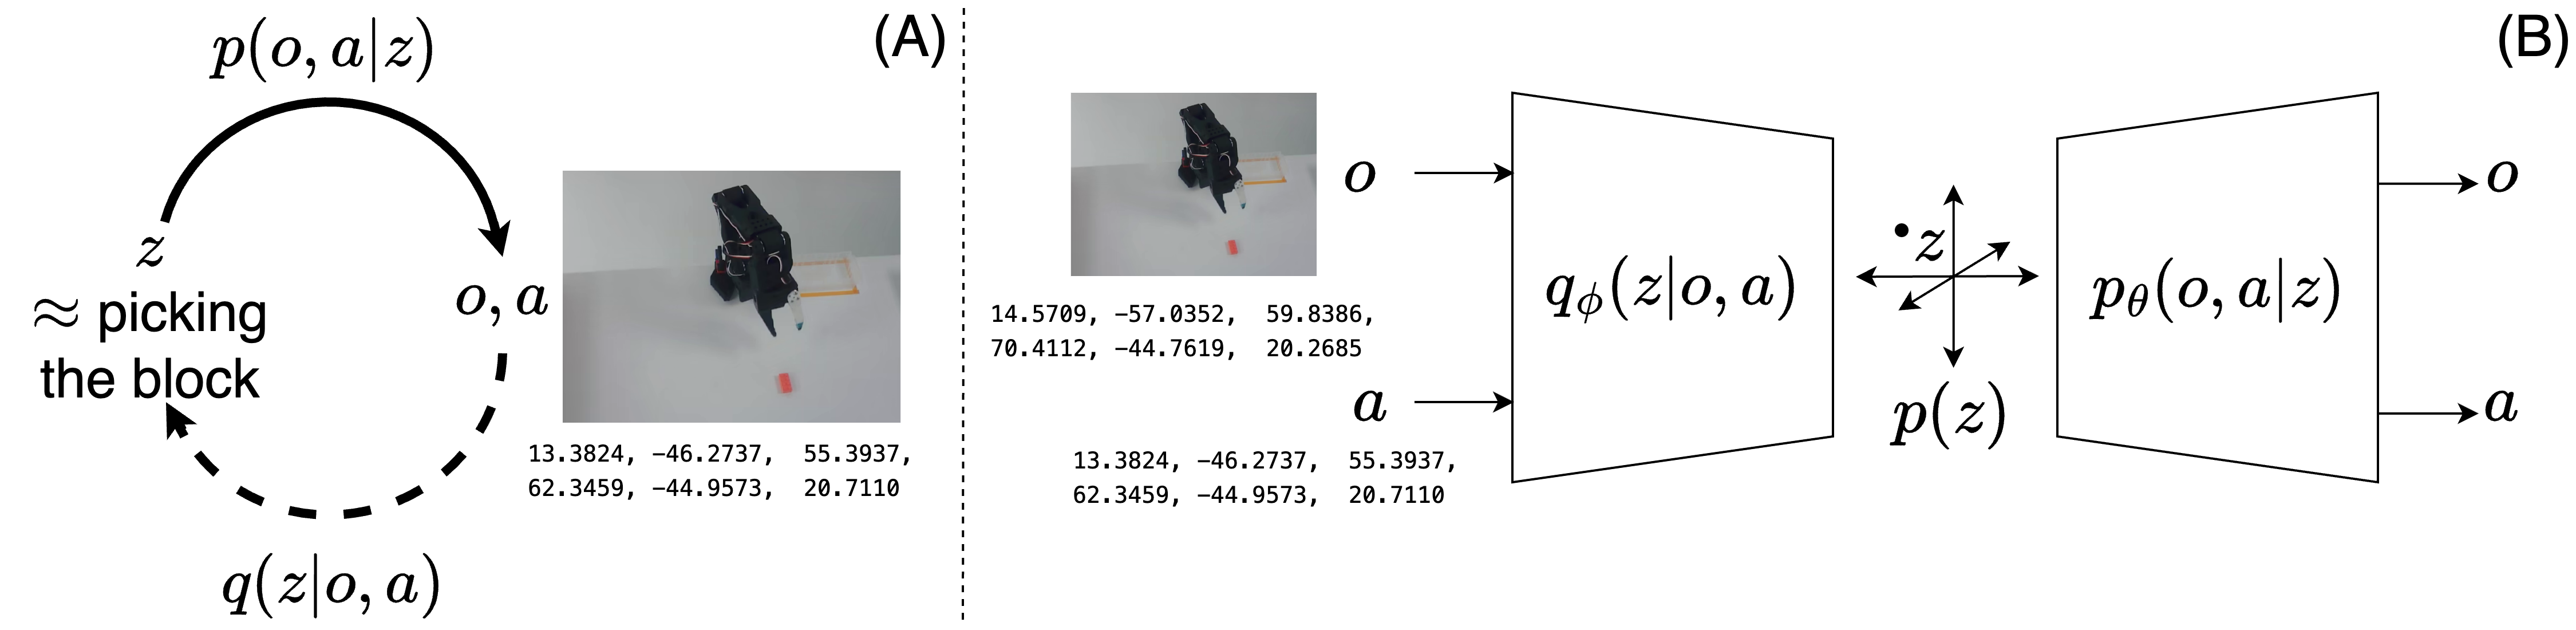
\includegraphics[width=0.9\textwidth]{figures/ch4/ch4-latent-variable-model.png}
    \caption{(A) The latent variable model in a robotics application regulates influence between observed (\(o,a) \) variables and an unobservable latent variable. (B) VAEs approximate exact latent variable models by means of variational inference. }
    \label{fig:ch4-latent-variable-model}
\end{figure}

Given a dataset \( \mathcal D \) consisting of \( N \) i.i.d. observation-action pairs, the log-likelihood of all datapoints under \( \theta \) (in Bayesian terms, the \emph{evidence} \( p_\theta(\mathcal D)\)) can thus be written as:
\begin{align}
    \log p_\theta(\mathcal D) &= \log \sum_{i=0}^N p_\theta ((o,a)_i) \label{eq:evidence-definition-1}\\
                              &= \log \sum_{i=0}^N \int_{\supp{Z}} p_\theta((o,a)_i \vert z) p(z) \label{eq:evidence-definition-2}\\
                              &= \log \sum_{i=0}^N \int_{\supp{Z}} \frac{q_\theta(z \vert (o,a)_i)}{q_\theta(z \vert (o,a)_i)} \cdot p_\theta((o,a)_i \vert z) p(z) \label{eq:evidence-definition-3}\\
                              &= \log \sum_{i=0}^N \mathbb E_{z \sim p_\theta(\bullet \vert (o,a)_i)} \left[ \frac{p(z)}{q_\theta(z \vert (o,a)_i)} \cdot p_\theta((o,a)_i \vert z) \right], \label{eq:evidence-definition}
\end{align}
where we used~\ref{eq:BC-latent-variable} in~\ref{eq:evidence-definition-1}, multiplied by \(1 = \frac{q_\theta(z \vert (o,a)_i)}{q_\theta(z \vert (o,a)_i)} \) in~\ref{eq:evidence-definition-2}, and used the definition of expected value in~\ref{eq:evidence-definition}.

In the special case where one assumes distributions to be tractable, \( p_\theta (\mathcal D) \) is typically tractable too, and \(\max_\theta \log p_\theta(\mathcal D) \) provides a natural target for (point-wise) infering the unknown parameters \( \theta \) of the generative model.
Unfortunately,~\ref{eq:evidence-definition} is rarely tractable when the distribution \( p \) is modeled with approximators such as neural networks, especially for high-dimensional, unstructured data.

In their seminal work on Variational Auto-Encoders (VAEs),~\citet{kingmaAutoEncodingVariationalBayes2022} present two major contributions to learn complex latent-variable GMs on unstructured data, proposing (1) a tractable, variational lower-bound to \ref{eq:evidence-definition} as an optimization target to jointly learn likelihood and posterior and (2) high-capacity function approximators to model the likelihood \(p_\theta(o,a\vert z)\) and (approximate) posterior distribution \( q_\phi(z \vert o,a) \approx q_\theta(z \vert o,a) \).

In particular, the lower bound on~\ref{eq:evidence-definition} (Evidence LOwer Bound, \emph{ELBO}) can be derived from~\ref{eq:evidence-definition} applying Jensen's inequality---\(\log \mathbb{E}[\bullet] \geq \mathbb{E} [\log (\bullet)] \)---yielding:
\begin{align}
    \log p_\theta(\mathcal D) &\geq \sum_{i=0}^{N} \left(
            \mathbb{E}_{z \sim p_\theta(\cdot \vert (o,a)_i)} \big[ \log p_\theta((o,a)_i \vert z) \big]
            + \mathbb{E}_{z \sim p_\theta(\cdot \vert (o,a)_i)} \left[ \log \left( \frac{p(z)}{q_\theta(z \vert (o,a)_i)} \right) \right]
        \right) \\
        &= \sum_{i=0}^{N} \left(
            \mathbb{E}_{z \sim p_\theta(\cdot \vert (o,a)_i)} \big[ \log p_\theta((o,a)_i \vert z) \big]
        - \DKL \big[ q_\theta(z \vert (o,a)_i) \Vert p(z) \big]
        \right) \label{eq:ELBO-intractable}
\end{align}
The true, generally intractable posterior \( p_\theta (z \vert o,a) \) prevents computing both the expectation and KL divergence terms in~\ref{eq:ELBO-intractable}, and therefore~\citet{kingmaAutoEncodingVariationalBayes2022} propose deriving the ELBO using an \emph{approximate} posterior \( q_\phi(z \vert o,a) \), resulting in the final, tractable ELBO objective,
\begin{align}
\text{ELBO}_{\mathcal D}(\theta, \phi) = \sum_{i=0}^{N} \left(
            \mathbb{E}_{z \sim q_\phi(\cdot \vert (o,a)_i)} \big[ \log p_\theta((o,a)_i \vert z) \big]
        - \DKL \big[ q_\phi(z \vert (o,a)_i) \Vert p(z) \big]
        \right)
        \label{eq:ELBO}
\end{align}
From Jensen's inequality, maximizing ELBO results in maximizing the log-likelihood of the data too, thus providing a natural, tractable optimization target.
Indeed, expectations can be estimated using MC estimates from the learned distributions in~\ref{eq:ELBO}, while the KL-divergence term can typically be computed in closed-form (1) modeling  \(q_\phi \) as a Gaussian \(q_\phi(z \vert o,a) = \mathcal N\big(\mu_\phi(o,a), \Sigma_\phi(o,a) \big) \) and (2) imposing a standard Gaussian prior on the latent space, \( p(z) = \mathcal N(\mathbf{0}, \mathbf{I}) \).

An intuitive explanation of the learning dynamics of VAEs can be given considering the equivalent case of \emph{minimizing the negative ELBO}, which admits a particularly interpretable factorization

\begin{align}
\min_{\theta, \phi} - \text{ELBO}_{\mathcal (o,a) \sim \mathcal D}(\theta, \phi) &= \min_{\theta, \phi}\mathbf{L^{\text{rec}}}(\theta) + \mathbf{L^{\text{reg}}}(\phi) \label{eq:VAE-min-neg-ELBO}\\
\mathbf{L^{\text{rec}}}(\theta) &= \mathbb{E}_{z \sim q_\phi(\cdot \vert o,a} \big[ \log p_\theta(o,a \vert z) \big] \label{eq:VAE-Lrec} \\
\mathbf{L^{\text{reg}}}(\phi) &= \DKL \big[ q_\phi(z \vert o,a) \Vert p(z) \big] \label{eq:VAE-Lreg}
\end{align}

For any given \((o,a) \) pair, the expected value term of~\ref{eq:VAE-Lrec} is typically computed via MC estimates, resulting in
\[ 
-\mathbb{E}_{z \sim q_\phi(\bullet \vert o,a)} \big[ \log p_\theta(o,a \vert z) \big] = \mathbf{L^{\text{rec}}} \approx - \frac{1}{n} \sum_{i=0}^n \log p_\theta(o,a \vert z_i).
\]
Assuming \( p_\theta(o,a \vert z) \) is parametrized as an isotropic Gaussian distribution with mean \(\mu_\theta (z) \in \mathbb R^d \) and variance \( \sigma^2 \), the log-likelihood thus simplifies to:
\[
\log p(o,a \vert z_i) = -\frac{1}{2\sigma^{2}} \big \Vert (o,a)-\mu_\theta(z_i) \big\Vert_2^2 -\frac{d}{2}\log(2\pi \sigma^{2}) \implies \mathbf{L^\text{rec}} \approx \frac {1}{n} \sum_{i=0}^n \big\Vert (o,a) - \mu_\theta(z_i) \big \Vert^2_2
\]
Indeed, it is very common in practice to approximate from the learned likelihood \( p_\theta(o,a \vert z) \) as a parametric distribution (e.g. Gaussians) parametrized by some learned vector of coefficients derived from \(\mu_\theta (z), \ z \sim p (\bullet) \).
In all such cases, learning a VAE corresponds to optimally \emph{reconstructing} the examples in \( \mathcal D \) by minimizing the L2-error---a very common \emph{supervised learning} objective for regression targets---while regularizing the information compression into the latent, as under the common modeling choice \( p(z) = \mathcal N (\mathbf{0}, \mathbf{I}) \)~\ref{eq:VAE-Lreg} regularizes the posterior limiting the expressivity of \( q_\phi(z\vert o,a) \).

% Diffusion
\paragraph{Diffusion Models}
VAEs approximate probability distributions via a \emph{single} latent variable model, assuming the underlying unknown distribution can be factored according to~\ref{eq:BC-latent-variable}, and solve the variational inference problem of jointly learning the likelihood \( p_\theta \) and (approximate) posterior \( q_\phi \) for such model.
In that, the unknown data distribution \( p(o,a) \) is effectively approximated via \( \int_Z p(z) p_\theta(o,a \vert z) \), and the underlying generative process reproduced by (1) sampling a latent variable and (2) learning to decode it into a (ideally) high-likelihood sample under the (unknown) \( p(o,a) \).
Diffusion Models (DMs)~\citep{hoDenoisingDiffusionProbabilistic2020} are another class of GMs which treat the similar problem of approximating an underlying unknown data distribution---\emph{variational inference}---by \emph{partially} extending VAEs to the case where \emph{multiple} latent variables influence each other and the generative process underlying \(o,a\) itself.
In particular, DMs posit the generative process can be decomposed to a series of piece-wise (Markovian) interactions between (latent) variables (Figure~\ref{fig:ch4-many-latents}), resulting in
\begin{align}
    p(\underbrace{o,a}_{= z_0}) &= \int_{\supp{Z_0}} \int_{\supp{Z_1}} \hdots \int_{\supp{Z_T}} p(z_0, z_1, \dots z_T) \label{eq:BC-multi-latent-model-1} \\ 
    p(z_0, z_1, \dots z_T) &= p(z_T) \prod_{t=0}^{T} p(z_{t-1} \vert z_t), \label{eq:BC-multi-latent-model-2}
\end{align}
where we explicitly showed the marginalization over the multiple latents in~\ref{eq:BC-multi-latent-model-1}, and used the law of conditional probability and Markov property in~\ref{eq:BC-multi-latent-model-2}.

\begin{figure}
    \centering
    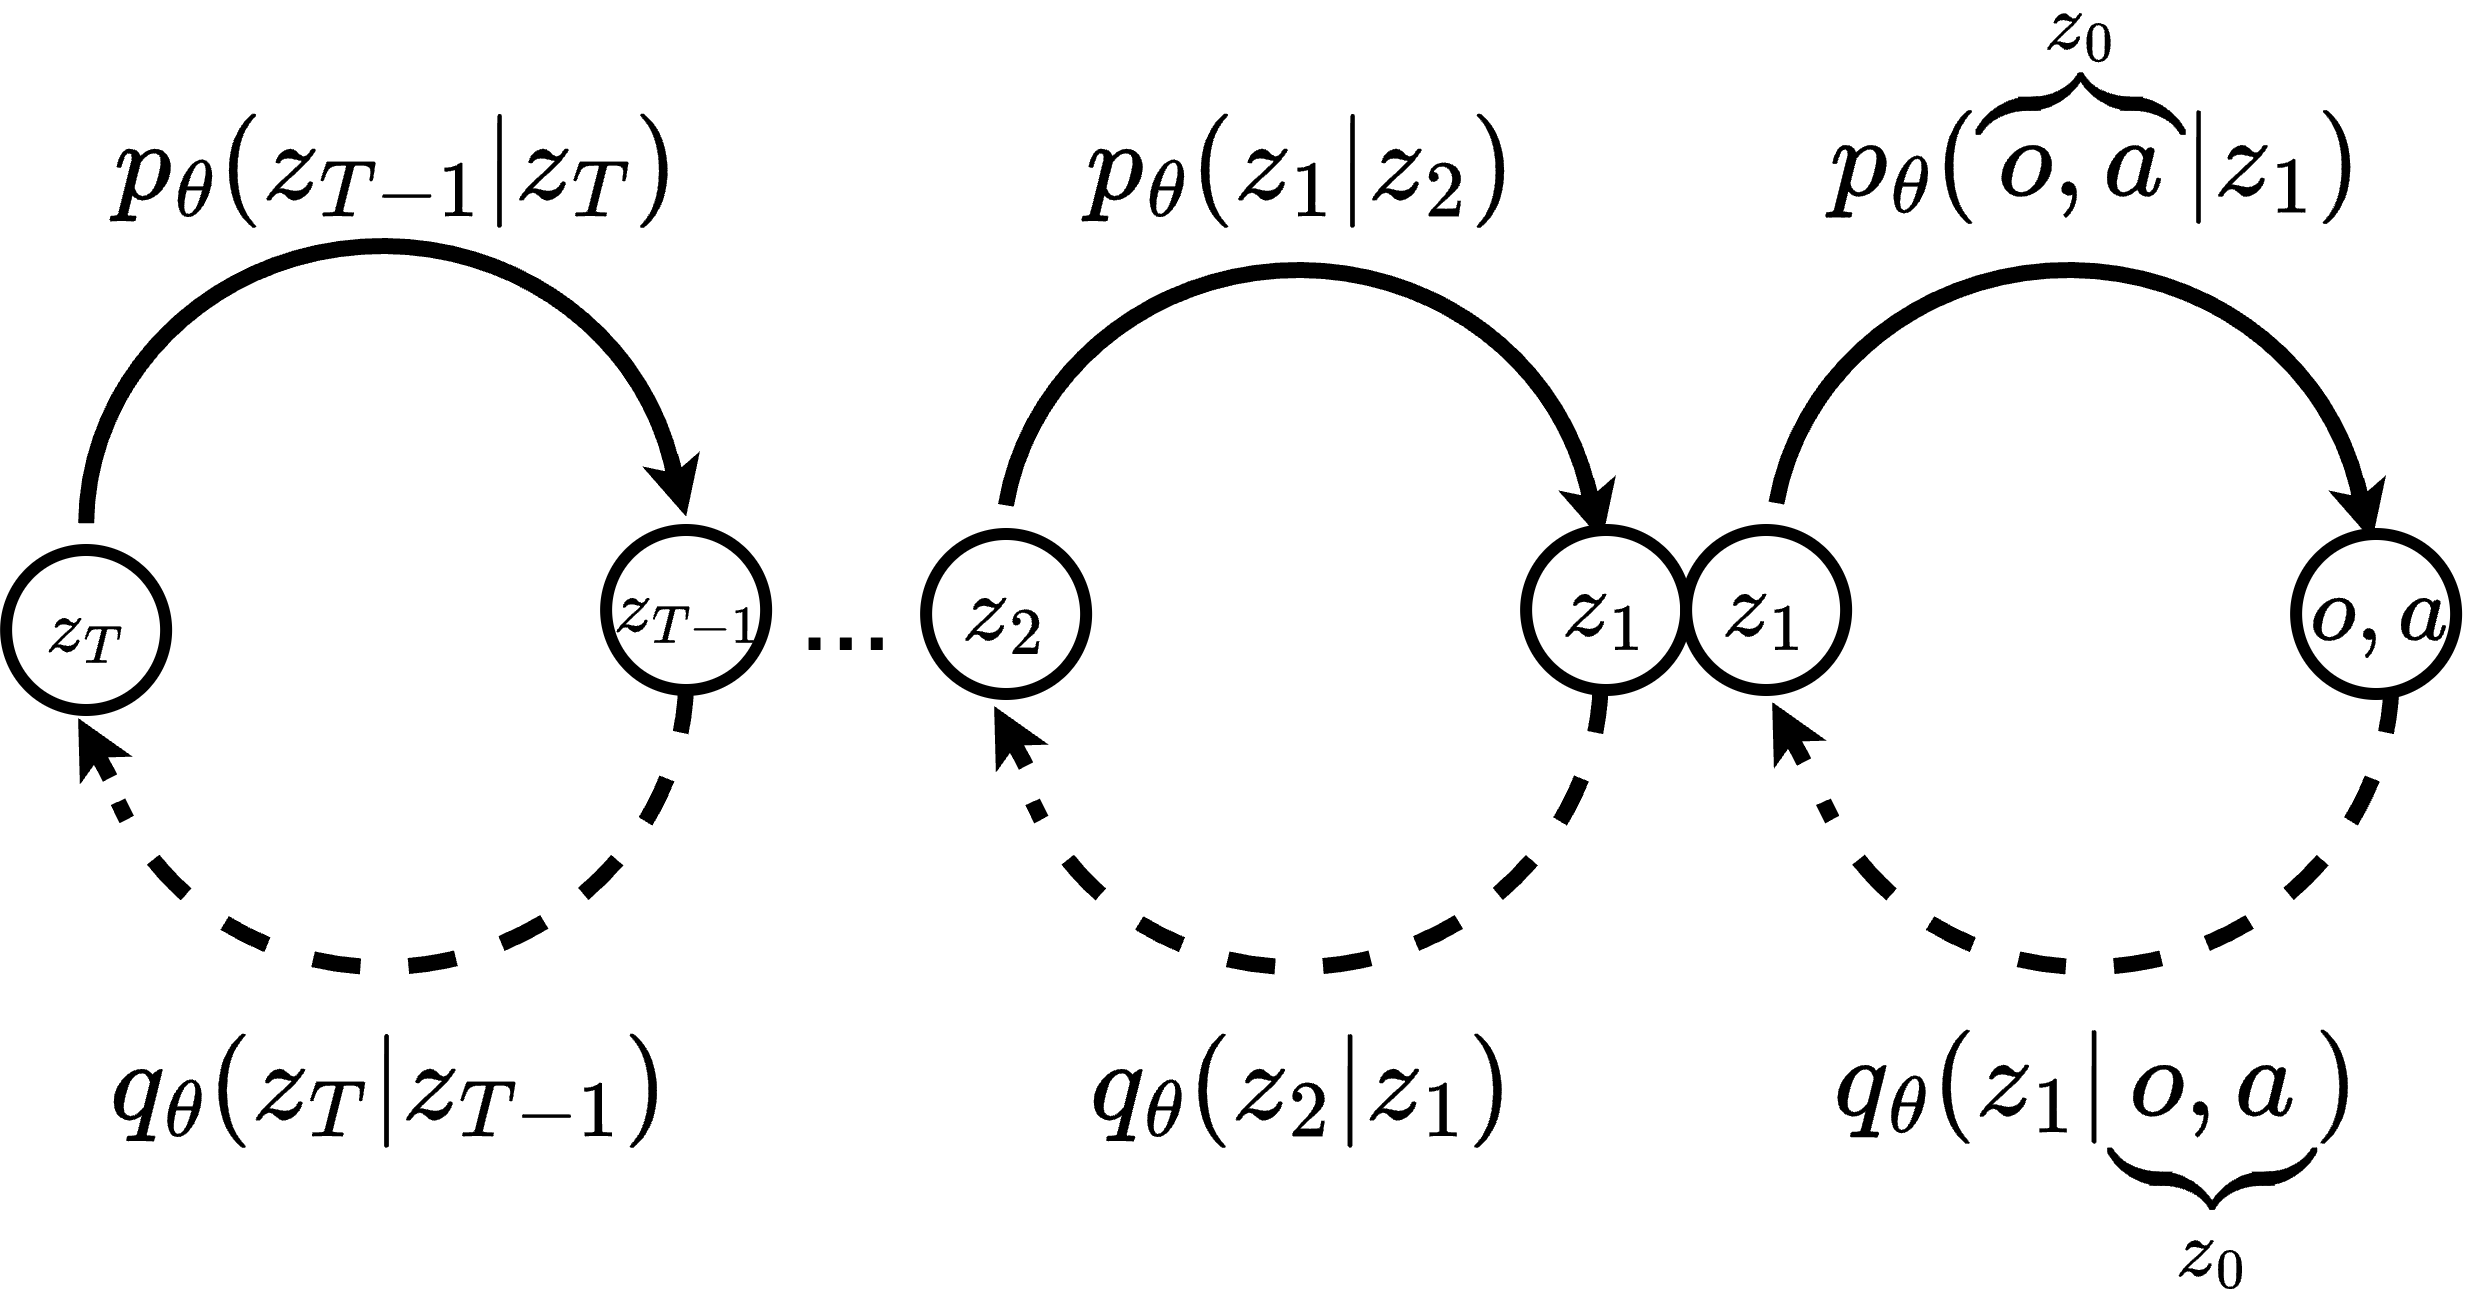
\includegraphics[width=0.5\textwidth]{figures/ch4/ch4-many-latents.png}
    \caption{HMLV models posit the data generation process is influenced by a stack of Markov-dependent latent variables, with samples from the posterior distribution being progressively higher up in the hierarchy.}
    \label{fig:ch4-many-latents}
\end{figure}

Similarily to VAEs, providing an exact interpretation for the latent variables is typically not possible.
Still, one fairly reasonable application-driven intuition is that, by providing a model of the hierarchical, decoupled interaction of latent variables, Hierarchical Markov Latent Variable (HMLV) models attempt to capture the different resolutions at which different conditioning factors intervene, so that in a robotics application for instance, one could naturally distinguish between early-stage trajectory planning (\( t \to T\)) and fine-grained adjustments (\( t \to 0 \)).
In that, HMLV models thus provide a framework to perform variational inference via multiple, sequential sampling steps from different higher level distributions instead of approximating the generative process with a single-latent variable model.
DMs are a particular instantiation of HMLV models for which the posterior \( q( z_t \vert z_{t-1}) = \mathcal N(z_t \sqrt{1-\beta_t}, \beta_t \mathbf{I}) \) for a given \( \beta_t \in \mathbb R^+ \), thereby iteratively reducing the signal-to-noise ratio as \( \beta_t \) increases along the latents hierarchy.

Just like VAEs, DMs attemp to learn to reproduce an underlying data distribution \( p (o,a) \) given a collection of i.i.d. samples approximating the model posited to have generated the data in the first place (~\ref{eq:BC-multi-latent-model-1}).
Similarily to VAEs, DMs approximate the process of sampling from the unknown \( p(o,a) \) (1) sampling from an easy-to-sample distribution (e.g., Gaussian) and (2) learning to reconstruct high-likelihood samples under the unknown distribution.
However, in stark contrast with VAEs, the easy-to-sample distribution contains \emph{no mutual information} regarding the data distribution \( p(o,a) \).
Crucially, as no information from the sample \( (o,a) \) (denoted as \( z_0 \equiv (o,a) \) for the sake of notation) is assumed to be propagated throughout the chain of latents, the posterior \( q(z_t \vert z_{t-1})\) assumes a relatively amicable structure in DMs, reducing complexity.
The \emph{true} likelihood \( p(z_{t-1} \vert z_t) \) is instead typically approximated using the parametrization \(  p_\theta (z_{t-1} \vert z_t) \).
In that, the information contained in the unknwon data distribution is \emph{reconstructed} via a process in which samples from a fixed distribution are turned into (ideally) high-likelihood samples under \( p(o,a) \)---a process referred to as \emph{denoising}.

Under such model, we can express the log-likelihood of an arbitrary sample as\footnote{\( o,a = z_0 \) for the sake of notation. Steps omitted for brevity. See Section A in~\citet{hoDenoisingDiffusionProbabilistic2020} for a complete derivation.
% See~\ref{appendix:diffusion-derivation}
}
\begin{align}
    \log p_\theta (\underbrace{o,a}_{= z_0}) = 
    &\mathbb{E}_{z_1 \sim q(\bullet \vert z_0)} \log p_\theta (z_0 \vert z_1) - \label{eq:diffusion-likelihood} \\
    &\mathbb{E}_{z_{T-1} \sim q(\bullet \vert z_0)} \big[ \DKL (q(z_T \vert z_{T-1}) \Vert p(z_T) ) \big] - \notag \\ 
    &\sum_{t=1}^{T-1} \mathbb{E}_{(z_{t-1}, z_{t+1}) \sim q(\bullet \vert z_0)} \big[ \DKL (q(z_t \vert z_{t-1}) \Vert p_\theta(z_t \vert z_{t-1}) ) \big], \notag
\end{align}
providing an optimization target in the form of \( \max_\theta \log p_\theta (\mathcal D) \).

In their seminal work on using DMs for variational inference,~\citet{hoDenoisingDiffusionProbabilistic2020} introduce major contributions regarding solving \( \min_\theta -\log p_\theta(o,a) \).
In particular,~\citet{hoDenoisingDiffusionProbabilistic2020} exclusively adopt a fixed \emph{Gaussian} posterior in the form of \( q(z_t \vert z_{t-1}) = \mathcal{N}(\sqrt{1-\beta_t}z_{t-1}, \beta_t \mathbf I) \).
The choice of adopting Gaussians has profound implications on the generative process modeled. 
Indeed, under the (mild) assumption that the variance is sufficiently small \( \beta_t \leq \eta, \eta \in \mathbb R^+ \),~\citet{sohl-dicksteinDeepUnsupervisedLearning2015} proved that the likelihood \( p(z_{t-1} \vert z_t) \) is Gaussian as well, which allows for the particularly convenient parametrization of the approximate likelihood \( p_\theta (x_{t-1} \vert x_t) = \mathcal N(\mu_\theta(x_t, t), \Sigma_\theta(x_t,t)), \ t \in [1,T] \), as well as for closed-form tractability of the KL-divergence terms in~\ref{eq:diffusion-likelihood}.
Further, the posterior's structure also enables an analytical description for the distribution of the \( t\)-th latent variable, \( q(z_t \vert z_0) = \mathcal N (\sqrt{\bar{\alpha}_t}z_0, (1-\bar{\alpha}_t) \mathbf{I}) \), with \( \alpha_t = 1-\beta_t, \ \bar \alpha_t = \prod_{k=1}^t \alpha_k \), which conveniently prevents iterative posterior sampling.

\begin{figure}
    \centering
    \includegraphics[width=0.9\textwidth]{figures/ch4/ch4-diffusion-robot-actions.png}
    \caption{DMs iteratively corrupt samples (left) from an unknown distribution into a quasi-standard Gaussian (center), learning the displacement field (right) that permits to reconstruct samples from the unknown target distribution by iteratively denoising samples of a tractable, easy-to-sample distribution.}
    \label{fig:diffusion-robot-actions}
\end{figure}

Finally, adopting Gaussian posteriors permits a particularly pleasing interpretation of the dynamics of training DMs~\citep{permenterInterpretingImprovingDiffusion2024}.
By using Gaussian posteriors, the hierarchical latent variables effectively lose increasingly more information circa the original (unknown) distribution's sample, \( z_0 \), increasingly distributing according to a standard Gaussian and thus containing no information at all (Figure~\ref{fig:diffusion-robot-actions}).
Figure~\ref{fig:diffusion-robot-actions} illustrates this procedure on a simplified, bidimensional observation-action distribution, where we considered \( o=q_2\) and \( a=q^h_2\), with \( q_2 \) representing the robot's \emph{elbow flex} actuation and \( q^h_2 \) the human teleoperator's robot elbow flex.

\begin{figure}
    \centering
    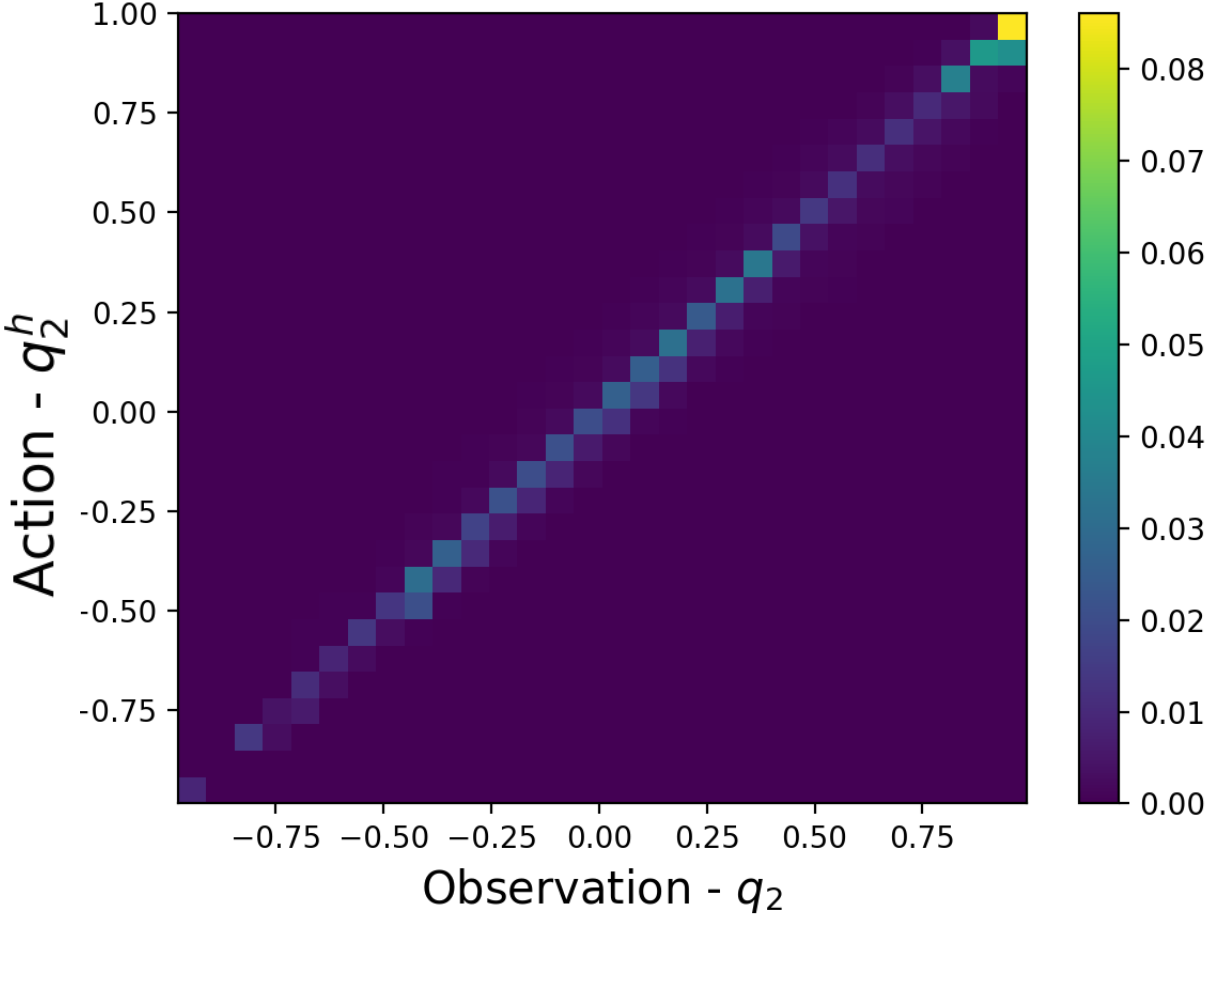
\includegraphics[width=0.3\textwidth]{figures/ch4/ch4-action-vs-observation-distribution.png}
    \caption{A joint action-observation distribution, in the simplified case where the observation is the elbow-flex actuation in a SO-100, and the action is the recorded position for the same joint in the teleoperator arm. The motion recorded being teleoperated, the points distribute along a the diagonal.}
    \label{fig:ch4-action-vs-observation-distribution}
\end{figure}

Because the recorded behavior is teleoperated, measurements mostly distribute along the line \( a = o + \eta, \eta \sim N(0,1) \), with \( \eta \)-variability accouting for minor control inconsistencies (Figure~\ref{fig:ch4-action-vs-observation-distribution}).
Using Gaussian posteriors---i.e., adding Gaussian noise---effectively simulates a \emph{Brownian motion} for the elements in the distribution's support (in Figure~\ref{fig:diffusion-robot-actions}, \( \obsspace \times \actionspace \)), whereby information \emph{diffuses away} from the samples, and comparing the diffused samples to the original data points one can derive an estimate of the total displacement induced by diffusion.
Under the only assumption that the likelihood of the diffused samples is low under the original unknown data distribution, then one can effectively approximate the unkwown distribution by learning to \emph{reverse} such displacement.
This key intuition allows to write a simplified training objective:
\begin{align}\label{eq:diffusion-simplified-loss}
    \mathcal L(\theta) = \mathbb{E}_{t, z_0, \epsilon} \big[
        \Vert \epsilon - \epsilon_\theta(\sqrt{\bar \alpha_t} z_0 + \epsilon \sqrt{1 - \bar \alpha_t}, t) \Vert^2 \big], \quad t \sim \mathcal{U}(\{1,\dots,T\}), \quad
        z_0 \sim \mathcal{D}, \quad
        \epsilon \sim \mathcal{N}(\mathbf{0},\mathbf{I}).
\end{align}

In this simplified (minimization) objective, the optimization process differs from~\ref{eq:diffusion-likelihood} in that, rather than maxizing \( p_\theta \) directly, the parameters \( \theta \) of the pairwise likelihood \( p_\theta(z_{t-1} \vert z_t) \) are adjusted to \emph{predict the total displacement} \( \epsilon \) for a randomly long (\( t \sim \mathcal{U}(\{1,\dots,T\} \) )) diffusion process starting from a sample of the target distribution.

By learning the total displacement from a generally, uninformative corrupted sample obtained diffusing information and a sample from an unknown distribution---significant (\( \Vert \epsilon \Vert > 0 \)) whenever input and target distribution are sufficiently different---~\citet{hoDenoisingDiffusionProbabilistic2020} show that one can approximate the underlying distribution reversing the displacement, \emph{denoising} samples.
Interestingly, under the hypothesis real-world data belongs to a single higher dimensional manifold (Manifold Hypothesis),~\citet{permenterInterpretingImprovingDiffusion2024} show that diffusion learns the gradient of a distance function from any off-point manifold (such as perturbed, uniformative samples), and the data manifold itself.
Following this gradient---i.e., denoising a sample from an uninformative distribution---corresponds to projecting back into the manifold, yielding a procedure to sample from unknown distributions by means of Euclidean projection.
Indeed, under the assumption that \(p_\theta (z_{t-1} \vert z_t) \) is Gaussian, then sampling \(z_{t-1} \sim p_\theta(\bullet \vert z_{t}) \) corresponds to computing
\begin{align}
    z_{t-1} = \frac{1}{\sqrt{\alpha_t}} \left( z_t - \frac{\beta_t}{\sqrt{1 - \bar\alpha_t}} \epsilon_\theta(z_t, t) \right) + \sigma_t \epsilon, \quad \epsilon \sim \mathcal N(\mathbf{0}, \mathbf{I}), \label{eq:diffusion-denoising-definition}
\end{align}
thus showing that the lower-level latent variables in a DM can be obtained by iteratively removing noise from the one-step higher order variable, using the noise regressor \( \epsilon_\theta(z_t, t)\) learned minimizing~\ref{eq:diffusion-simplified-loss}.

\subsection{Action Chunking with Transformers}
While GMs prove useful in learning complex, high-dimensional multi-modal distributions, they do not natively address the compouding errors problem characteristic of online, sequential predictions.
In Action Chunking with Transformers (ACT),~\citet{zhaoLearningFineGrainedBimanual2023} present an application of VAEs to the problem of learning purely from offline trajectories, introduce a simple, yet effective method to mitigate error compounding, learning high-fidelity autonomous behaviors.
Drawing inspiration from how humans plan to enact atomically sequences of the kind \( a_{t:t+k} \) instead of single actions \( a_t \),~\citet{zhaoLearningFineGrainedBimanual2023} propose learning a GM on a dataset of input demonstrations by modeling \emph{action chunks}.
Besides contributions to learning high-performance autonomous behaviors,~\citet{zhaoLearningFineGrainedBimanual2023} also introduce hardware contributions in the form of a low-cost bimanual robot setup (ALOHA) capable of performing fine-grained manipulation tasks, such as opening a lid, slotting a battery in its allotment or even prepare tape for application.

On the robot learning side of their contributions,~\citet{zhaoLearningFineGrainedBimanual2023} adopt transformers as the architectural backbone to learn a \emph{Conditional} VAE~\citep{sohnLearningStructuredOutput2015}. 
Conditional VAEs are a variation of the more standard VAE formulation introducing a conditioning variable on sampling from the latent prior, allowing the modeling of \emph{one-to-many} relationships between latent and data samples.
Further, in stark contrast with previous work~\citep{florenceImplicitBehavioralCloning2022,jannerPlanningDiffusionFlexible2022},~\citet{zhaoLearningFineGrainedBimanual2023} do not learn a full joint \( p_\theta(o,a) \) on observation and actions.
While the \emph{policy} distribution \( p_\theta(a \vert o) \) can in principle be entirely described from its joint \( p_\theta(o,a) \), it is often the case that the conditional distribution is intractable when using function approximators, as \( p_\theta(a \vert o) = \tfrac{p_\theta(o,a)}{\int_\actionspace p_\theta(o,a)} \) and the integral in the denominator is typically intractable.
Instead of modeling the full joint using a vanilla VAE,~\citet{zhaoLearningFineGrainedBimanual2023} propose learning a \emph{conditional} VAE~\citep{sohnLearningStructuredOutput2015} modeling the policy distribution directly \( p (a \vert o) \).

In practice, when learning from demonstrations adopting CVAEs results in a slight modification to the VAE objective in~\ref{eq:ELBO}, which is adapted to
\begin{align}\label{eq:c-ELBO}
    \text{ELBO}_{\mathcal D}(\theta, \phi, \omega) = \sum_{i=0}^{N} \left(
            \mathbb{E}_{z \sim q_\phi(\cdot \vert o_i, a_i)} \big[ \log p_\theta(a_i \vert z, o_i) \big]
        - \DKL \big[ q_\phi(z \vert o_i, a_i) \Vert p_\omega(z \vert o_i) \big]
        \right)
\end{align}
Notice how in~\ref{eq:c-ELBO} we are now also learning a new set of parameters \( \omega \) for the prior distribution in the latent space.
Effectively, this enables conditioning latent-space sampling (and thus reconstruction) during training, and potentially inference, providing useful when learning inherently conditional distributions like policies.
Further, ACT is trained as a \( \beta\)-CVAE~\citep{higgins2017beta}, using a weight of the KL regularization term in~\ref{eq:c-ELBO} as an hyperparameter regulating the information condensed in the latent space, where higher \( \beta \) results in a less expressive latent space.

In their work,~\citet{zhaoLearningFineGrainedBimanual2023} ablated using a GM to learn from human demonstrations compared to a simpler, supervised objective, \( \mathcal L_1(a,a^\prime) = \Vert a - a^\prime \Vert_1 \).
Interestingly, they found the performance of these two approaches to be comparable when learning from \emph{scripted} demonstrations.
That is, when learning from data collected rolling out a predetermined set of commands \( [q^c_0, q^c_1, \dots] \), GM did \emph{not} prove competitive compared to standard supervised learning.
However, when learning from human demonstrations---i.e., from data collected executing commands coming from a human controller \( [q^h_0, q^h_1, \dots] \)---they found performance (success rate on a downstream task) to be severily (-33.3\%) hindered from adopting a standard supervised learning objective compared to a richer, potentially more complex to learn variational objective, in keeping with the multimodal nature of human demonstrations data and findings presented in~\citet{florenceImplicitBehavioralCloning2022}.
The authors also ablate the action chunking paradigm, reporting significant performance gains for performing action chunking (1\% vs. 44\% success rate).
To avoid acting openloop,~\citet{zhaoLearningFineGrainedBimanual2023} design an inference process consisting in performing inference at every timestep \( t \) and then aggregate overlapping chunks using chunks' exponential moving average.

\begin{figure}
    \centering
    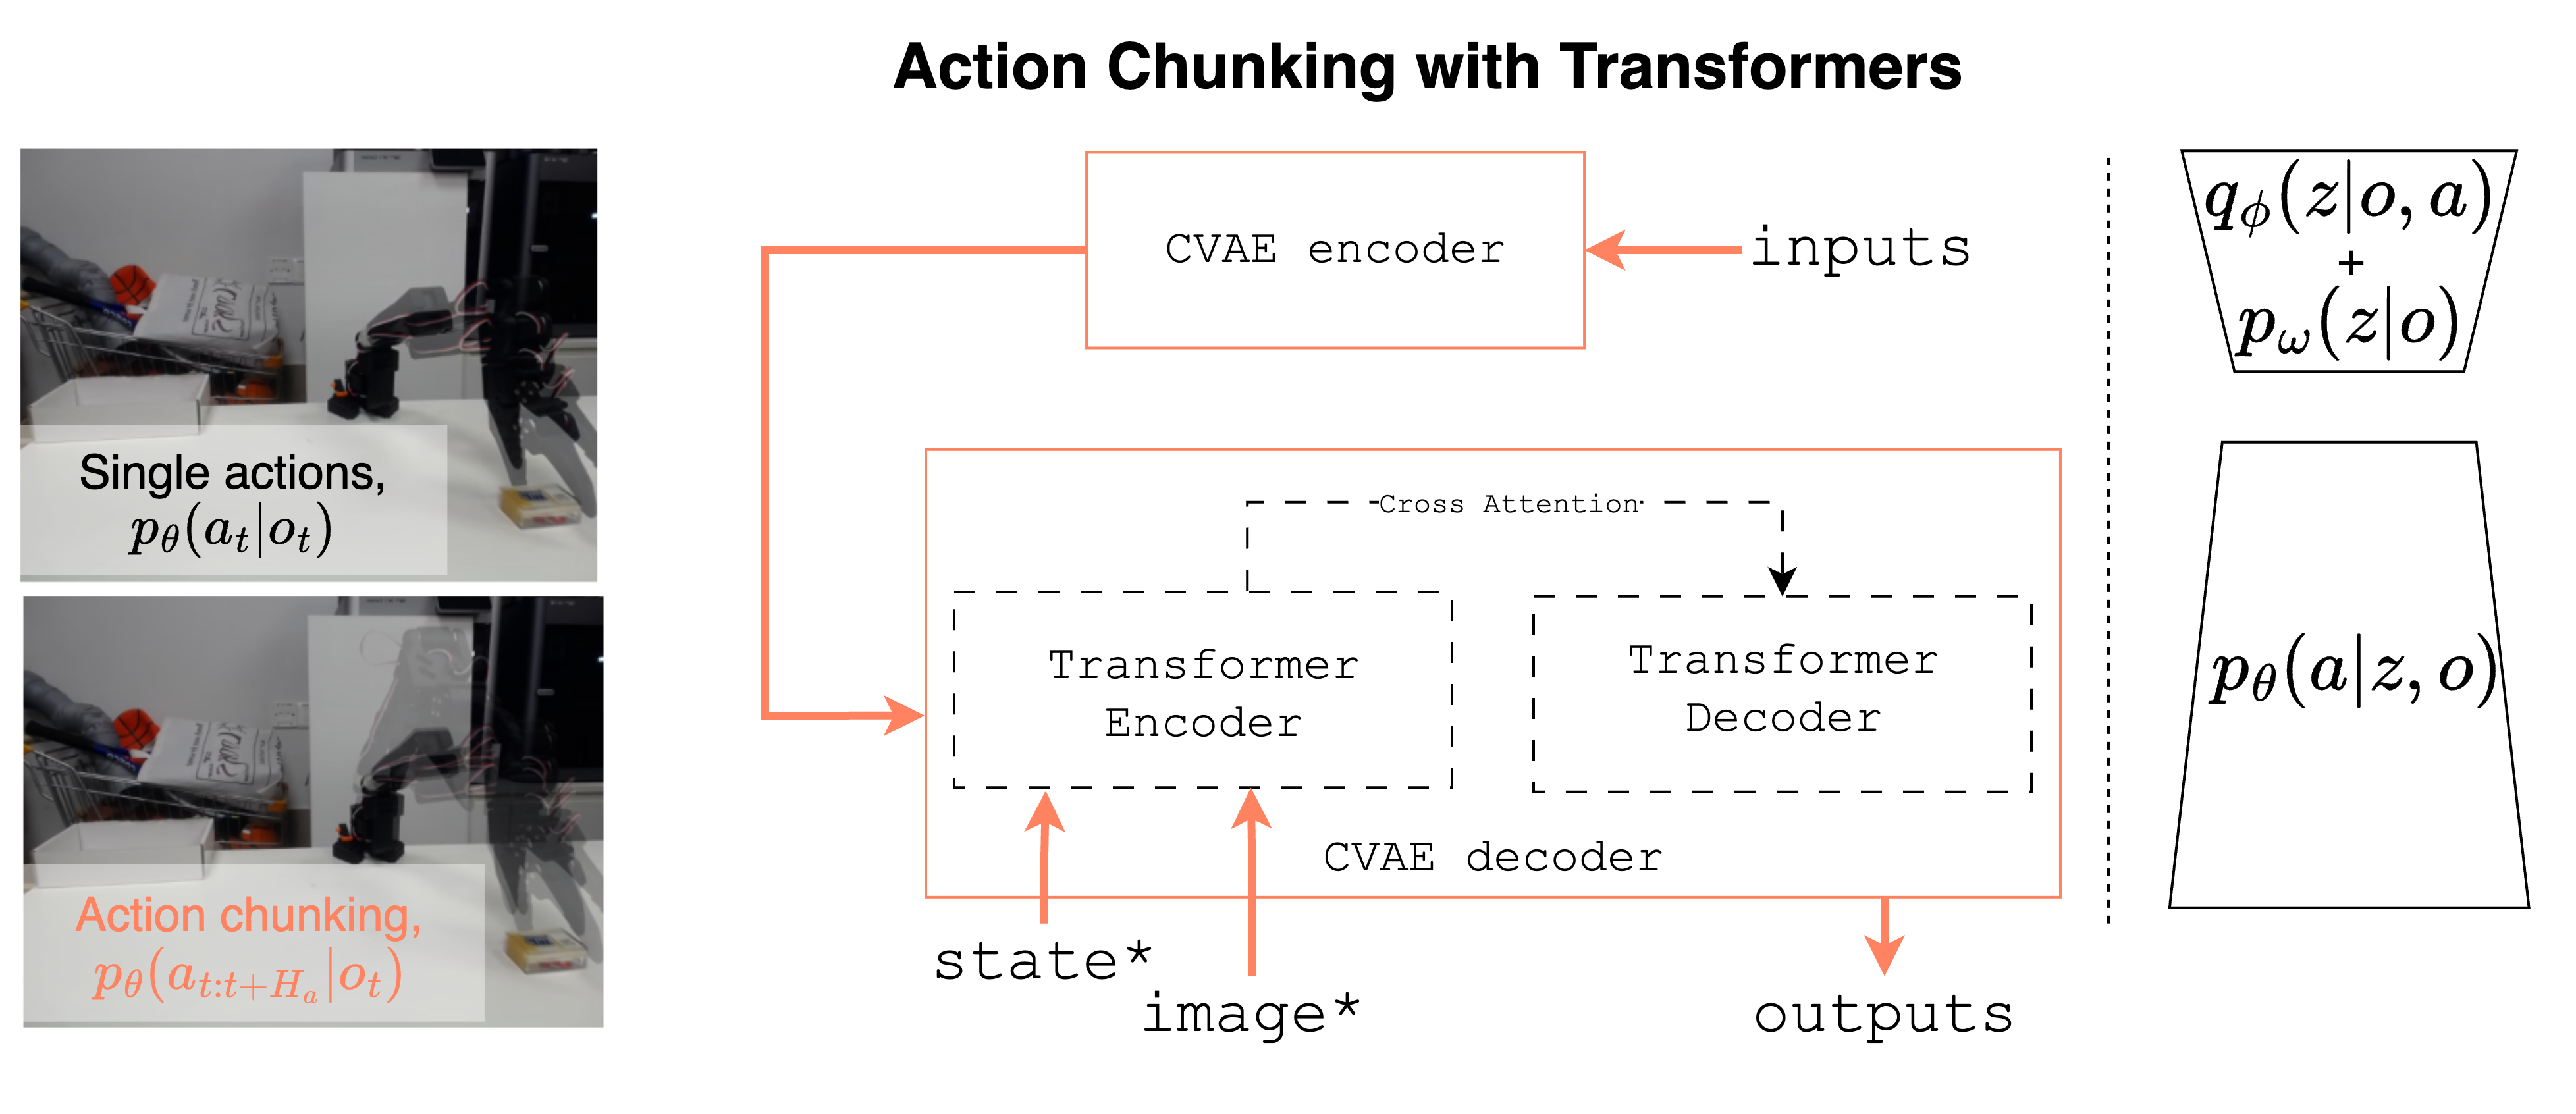
\includegraphics[width=0.9\textwidth]{figures/ch4/ch4-act.png}
    \caption{Action Chunking with Transformer (ACT), as in~\citet{zhaoLearningFineGrainedBimanual2023}. ACT introduces an action chunking paradigm to cope with high-dimensional multi-modal demonstration data, and a transformer-based CVAE architecture.}
    \label{fig:ch4-act}
\end{figure}

In ACT (Figure~\ref{fig:ch4-act}), inference for a given observation \( o \in \mathcal O \) could be performed by (1) computing a prior \( p_\omega(z \vert o) \) for the latent and (2) decoding an action chunk from a sampled latent \( z \sim p_\omega(\bullet \vert o) \), similarily to how standard VAEs generate samples, with the exception that vanilla VAEs typically pose \( p(z\vert o) \equiv p(z) \sim N(\mathbf{0}, \mathbf{I}) \) and thus skip (1).

\begin{figure}
    \centering
    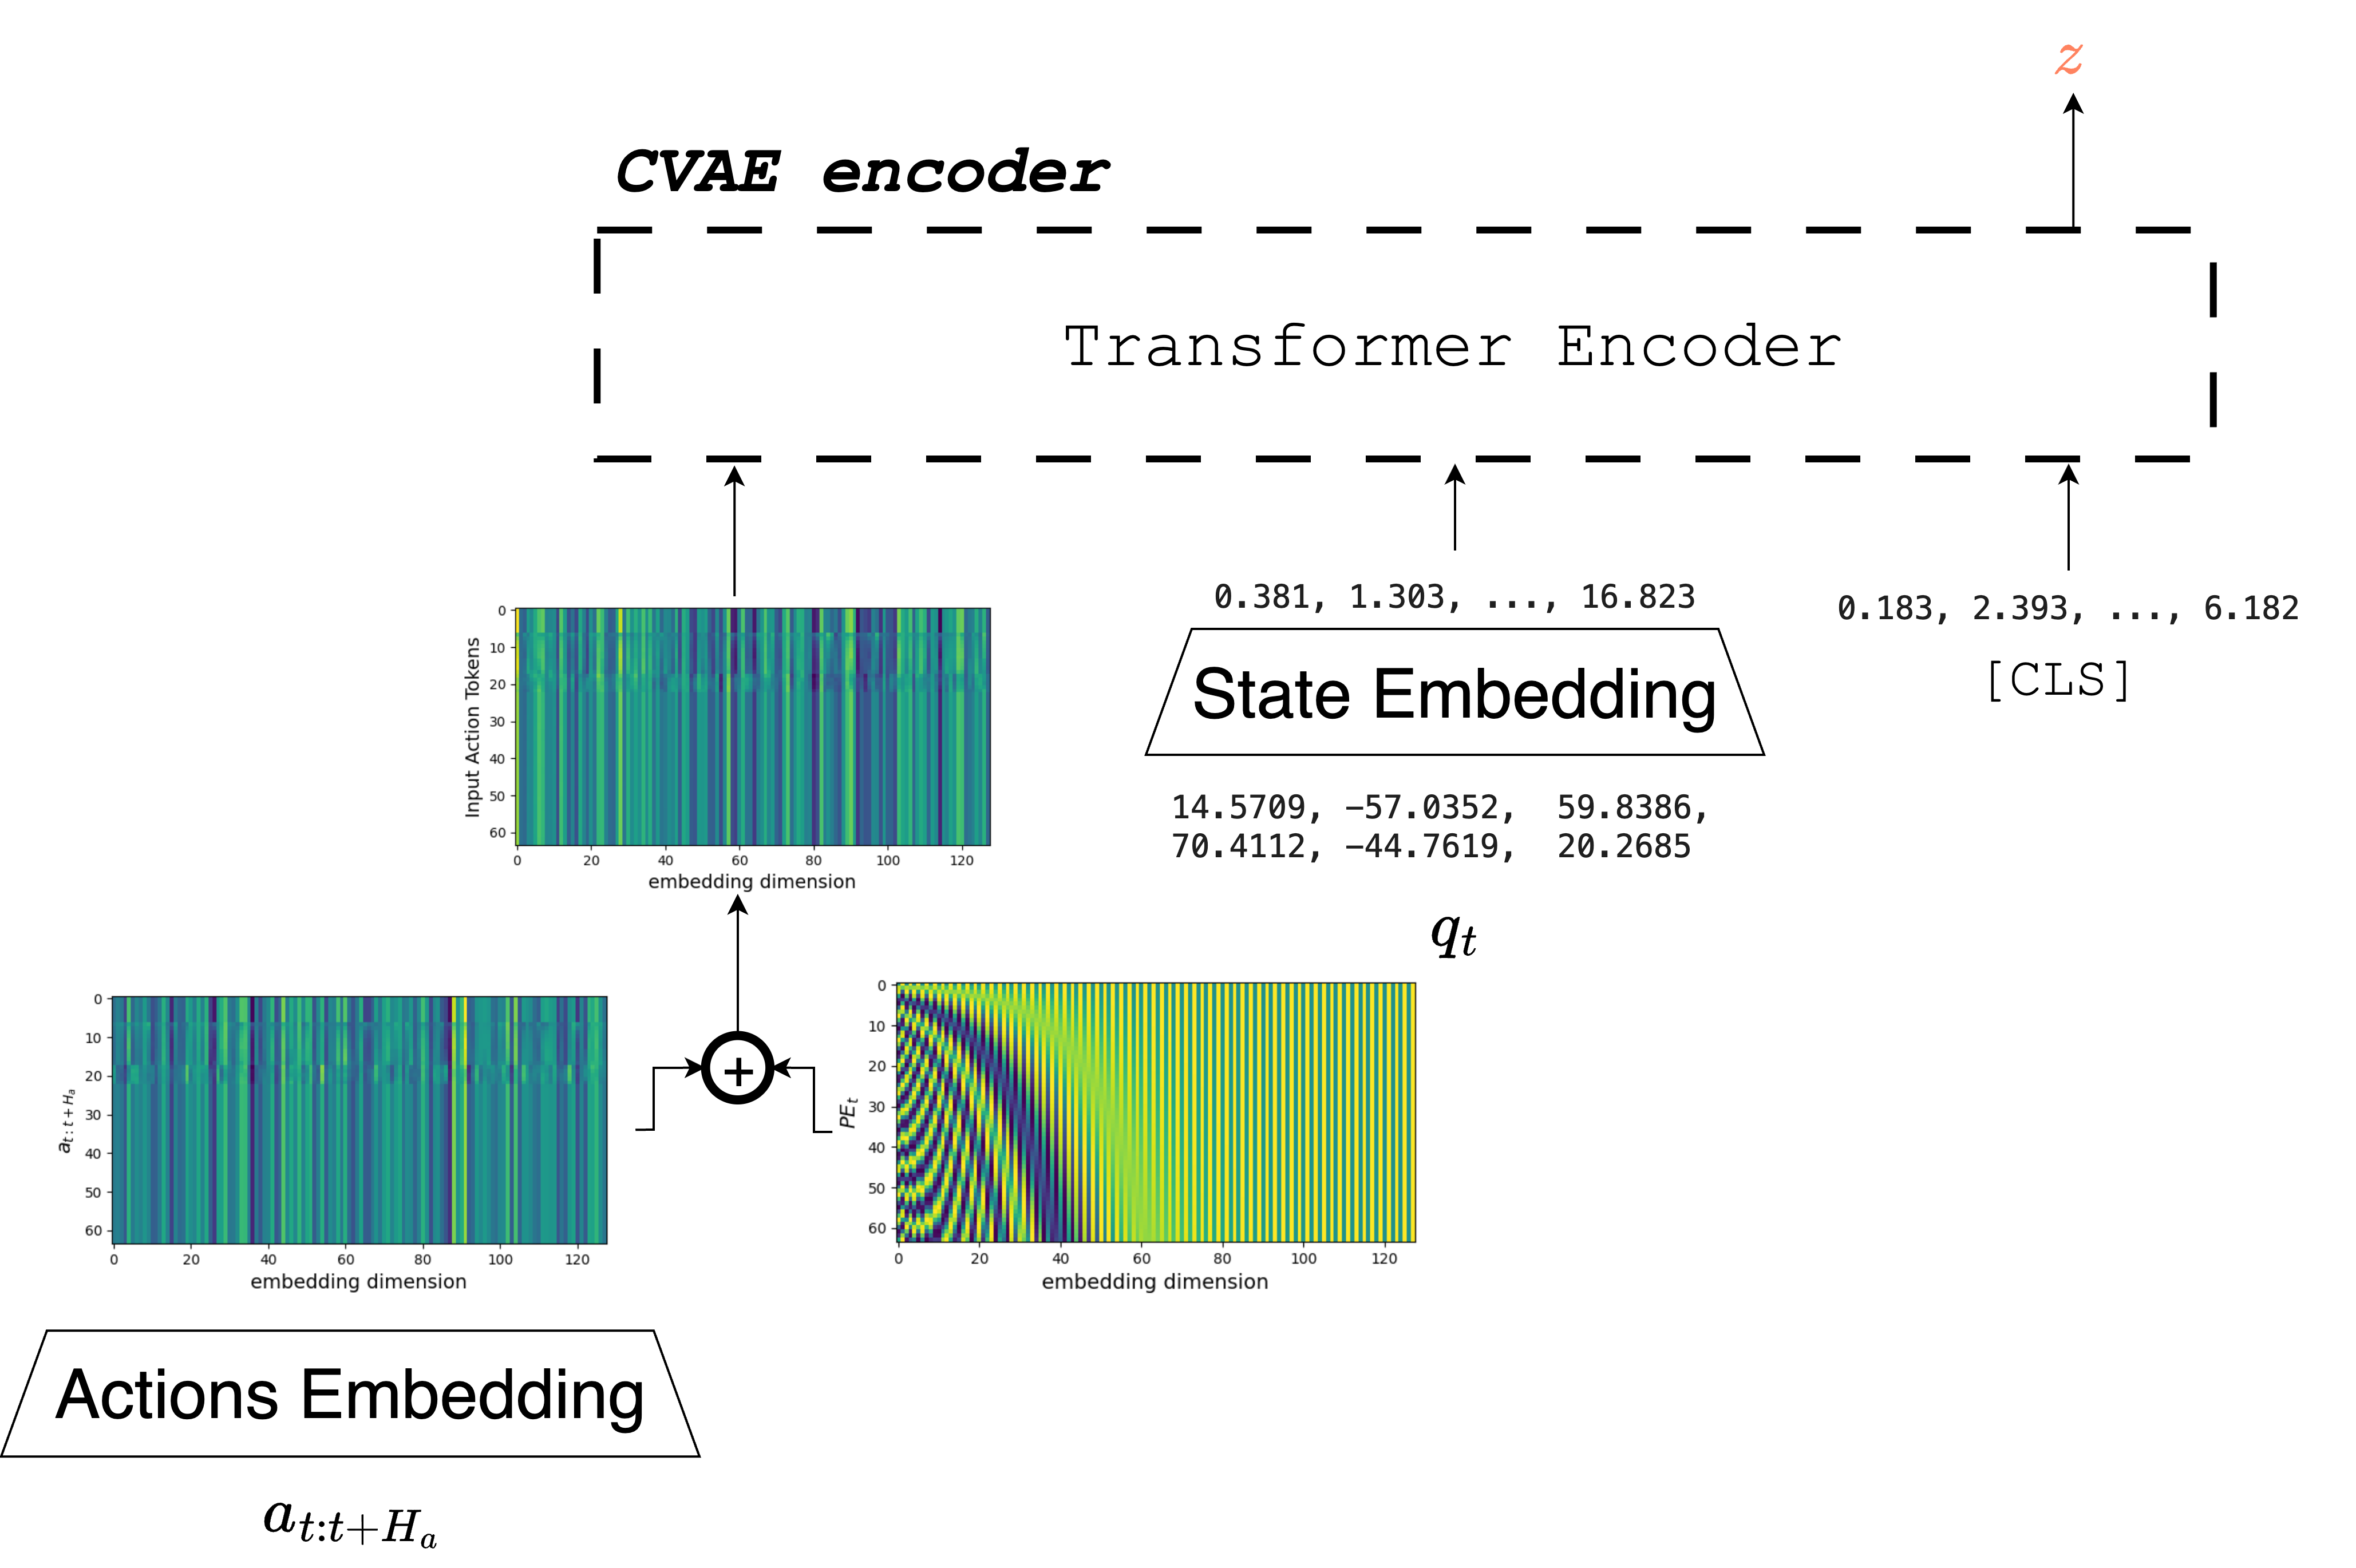
\includegraphics[width=0.75\textwidth]{figures/ch4/ch4-act-encoder.png}
    \caption{The CVAE encoder used in ACT. Input action chunks are first embedded and aggregated with positional embeddings, before being processed alongside embedded proprioperceptive information, and a learned \texttt{[CLS]} token used to aggregate input level information, and predict the style variable \( z \). The encoder is entirely disregarded at inference time.}
    \label{fig:ch4-act-encoder}
\end{figure}

However, the authors claim using a deterministic procedure to derive \( z \) may benefit policy evaluation, and thus avoid sampling from the conditional prior at all.
At test time, instead, they simply use \( z = \mathbf{0} \), as the conditional prior on \( z \) used in training is set to be the unit Gaussian.
At test time, conditioning on the observation \( o \) is instead achieved through explicitly feeding proprioperceptive and visual observations to the decoder, \( p_\theta(a \vert z, o) \), while during training \( z \) is indeed sampled from the approximate posterior distribution \(p_\phi(z \vert o, a)\), which, however, disregards image observations and exclusively uses proprioperceptive states to form \( o \) for efficiency reasons (as the posterior \(q_\phi \) is completely disregarded at test time).

\begin{figure}
    \centering
    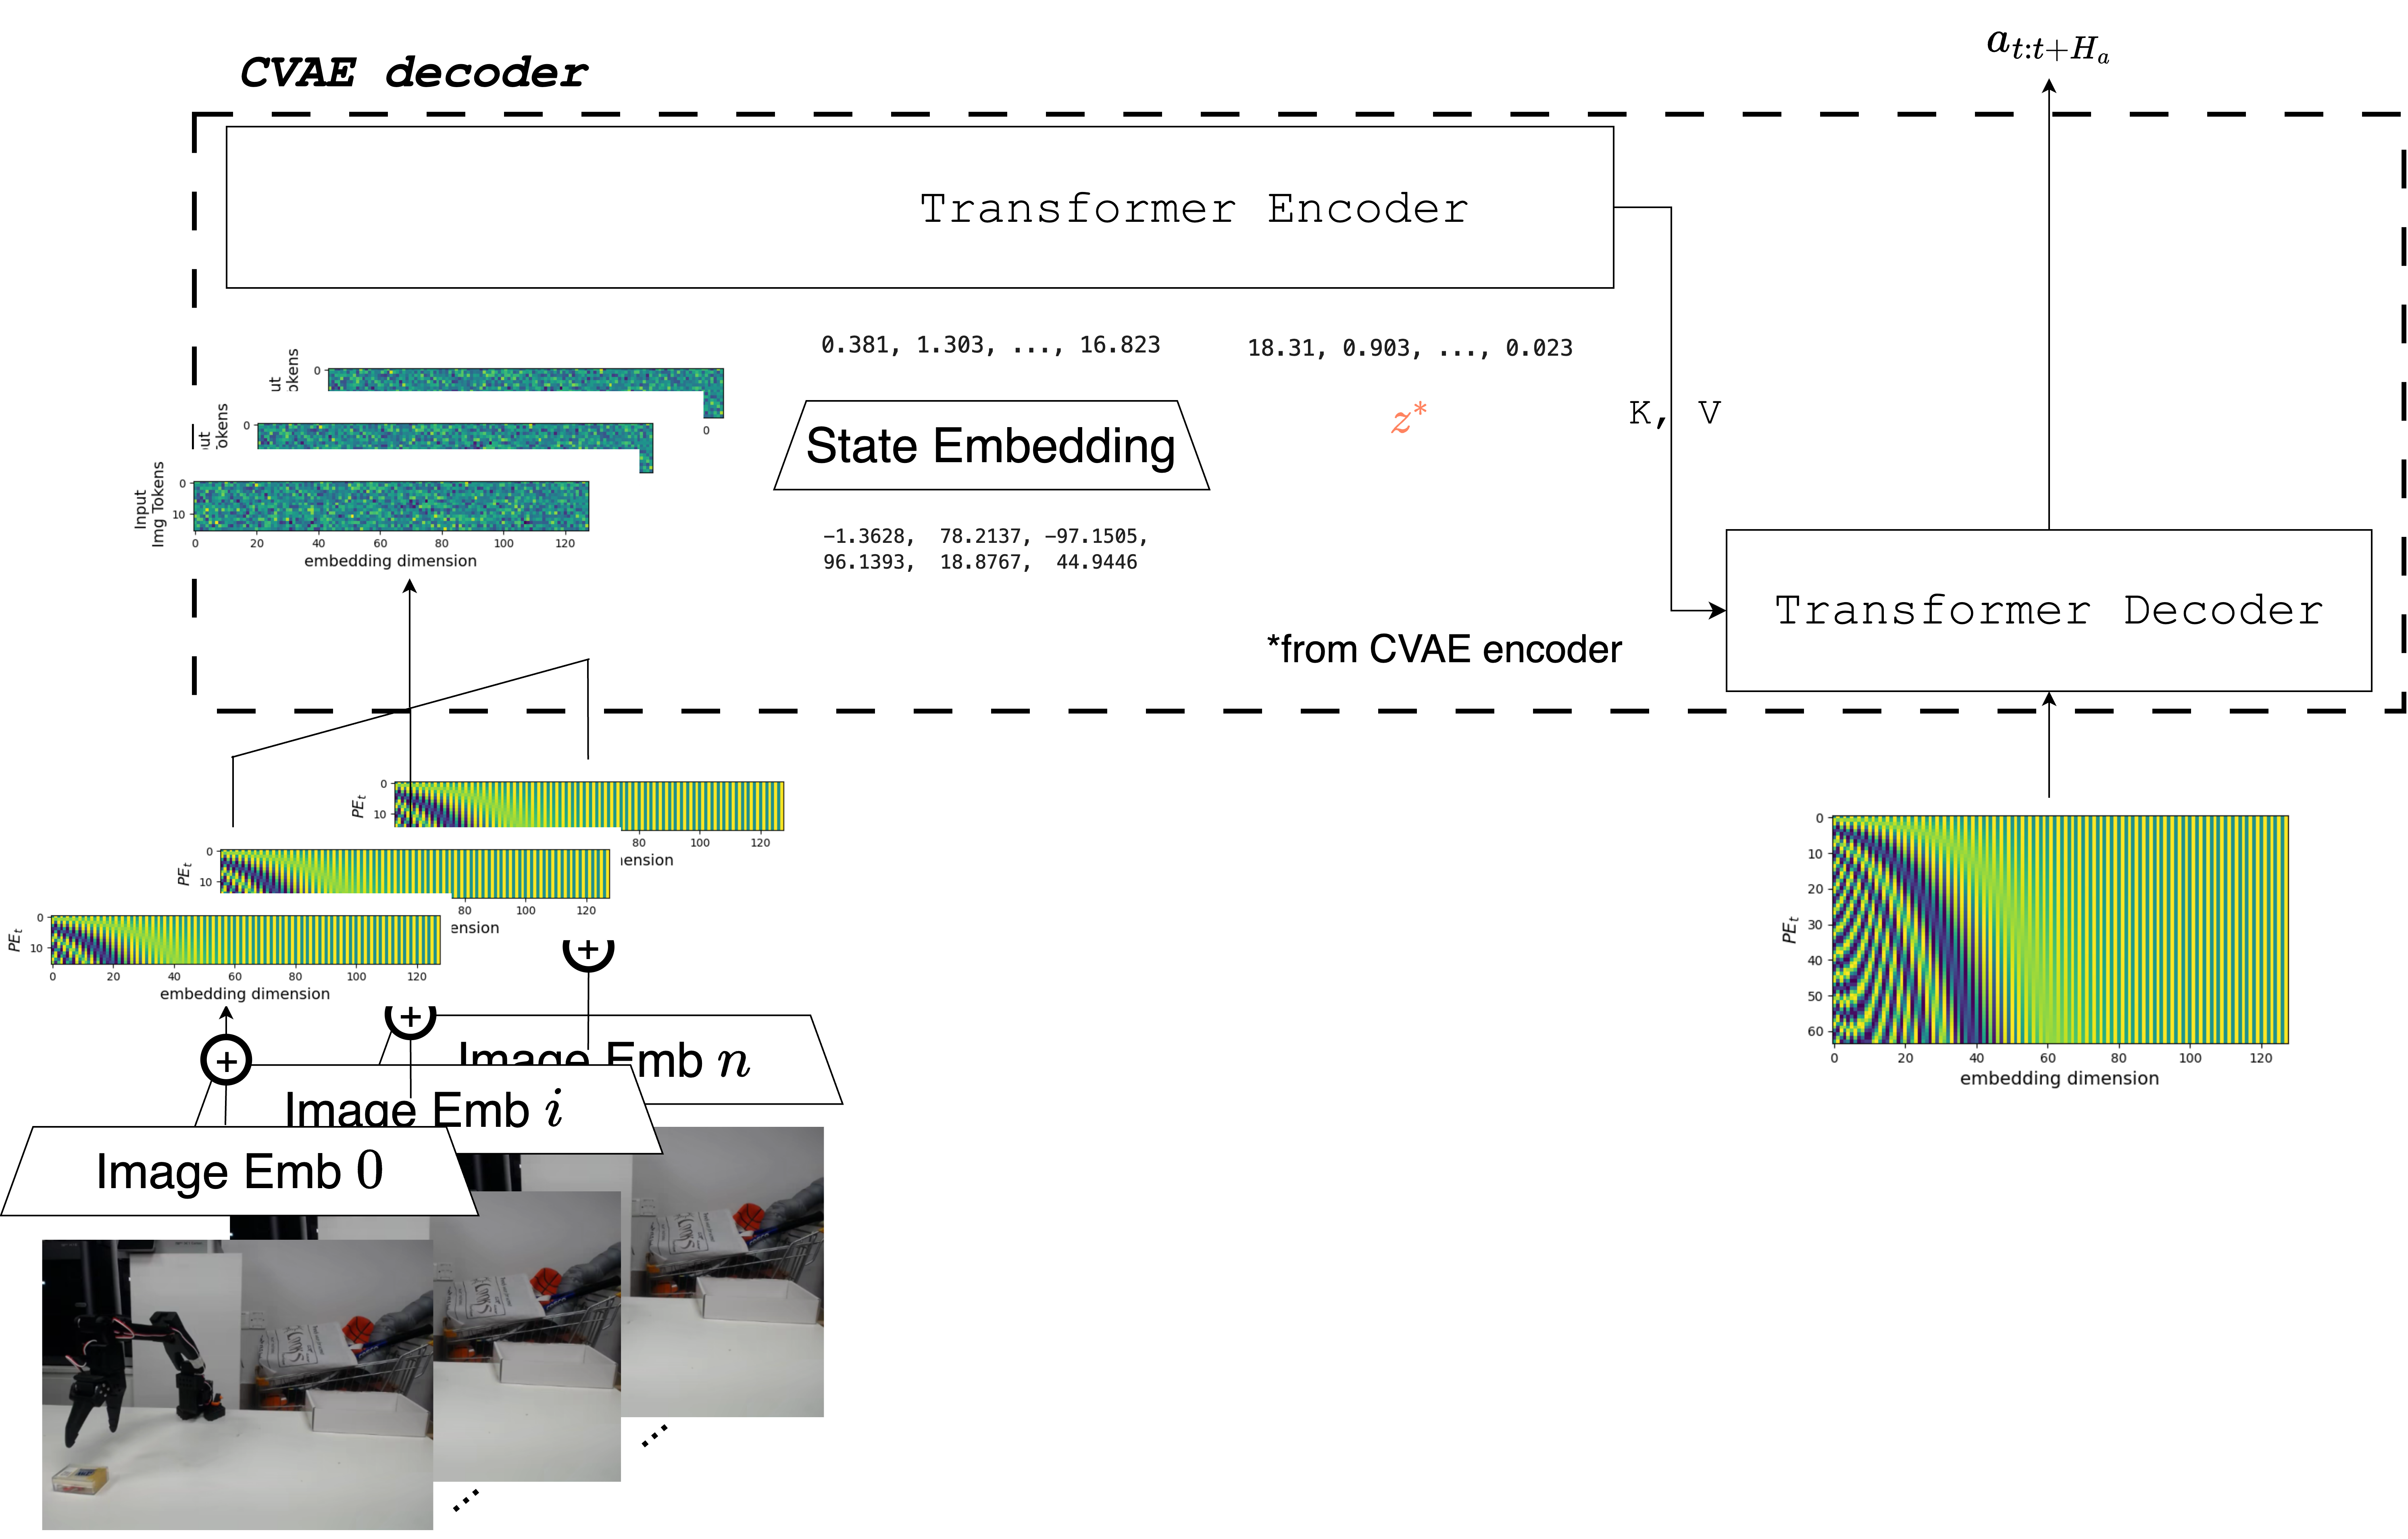
\includegraphics[width=0.75\textwidth]{figures/ch4/ch4-act-decoder.png}
    \caption{The CVAE decoder used in ACT, comprising of a full encoder-decoder Transformer architecture. Camera observations from all \( n \) camera views are first embedded using pre-trained visual encoders, and then concatenated to the corresponding positional embeddings. Then, alongside embeddings for the proprioperceptive information available and the style variable \(z\) retrieved from the CVAE encoder, the Transformer encoder shares the matrices \( K,Q \) with the Transformer decoder, trained to decode fixed position embeddings into action valid chunks.}
    \label{fig:ch4-act-decoder}
\end{figure}


\subsubsection{Code Example: Learning ACT}
\todo{using act example}

\subsection{Diffusion Policy}
DMs proved very effective in approximating complex highly dimensional distributions, such as distributions over images~\citep{hoDenoisingDiffusionProbabilistic2020} or videos~\citep{polyakMovieGenCast2025}, thanks to their inherent capability to deal with multimodal data and training stability.
In Diffusion Policy (DP),~\citet{chiDiffusionPolicyVisuomotor2024} present an application of DMs the field of robot learning, leveraging diffusion to model human expert demonstrations in a variety of simulated and real-world tasks.
Similarily to Action Chunking with Transformer~\citep{zhaoLearningFineGrainedBimanual2023},~\citet{chiDiffusionPolicyVisuomotor2024} (1) adopt a modified \emph{observation-conditioned target distribution} instead of the full joint \( p(o,a) \) and (2) predict multiple actions into the future instead of a single action.
Besides the intractability of the observations' marginal \( p_\theta(o) \) given \(p_\theta(o,a) \), DP's rationale for modeling the data distribution via \( p_\theta(a \vert o) \) stems from the rather test-time compute intensive nature of diffusion, whereby generating actions \emph{alongside} observations is likely to result in higher complexity and thus a likely larger number of denoising operations, which would prove ultimately pointless considering robotics applications rely on the capability to generate controls rather than reproducing observations.

In practice, conditioning on observation data is achieved conditioning the added noise regressor \( \epsilon_\theta \) introduced in~\ref{eq:diffusion-simplified-loss} on a stack of \( T_o \) observations, resulting in the \emph{conditional} simplified diffusion objective
\begin{align}
    \mathcal L(\theta) &= \mathbb{E}_{t, a_{t:t+H_a}, \epsilon} \big[
        \Vert \epsilon - \epsilon_\theta(\sqrt{\bar \alpha_t} a_{t:t+T_a} + \epsilon \sqrt{1 - \bar \alpha_t}, t, o_{t-T_o:t}) \Vert^2 \big], \label{eq:diffusion-policy-objective} \\
        & t \sim \mathcal{U}(\{1,\dots,T\}), \quad
        a_{t:t+T_a}, o_{t-T_o:t} \sim \mathcal{D}, \quad
        \epsilon \sim \mathcal{N}(\mathbf{0},\mathbf{I}). \notag 
\end{align}
Notice how in~\ref{eq:diffusion-policy-objective} the noise regressor is conditioned both on the latent variable rank \( t \) \emph{and} on a stack of previous observations \(o_{t-T_o:t} \).
~\citet{chiDiffusionPolicyVisuomotor2024} claim the combination of (1) conditioning on a horizon of previous observations and (2) predicting multiple actions into the future allows DP to \emph{commit to specific modes} in the data at inference time, which proves essential for good performance and avoiding undecisiveness.

\begin{figure}
    \centering
    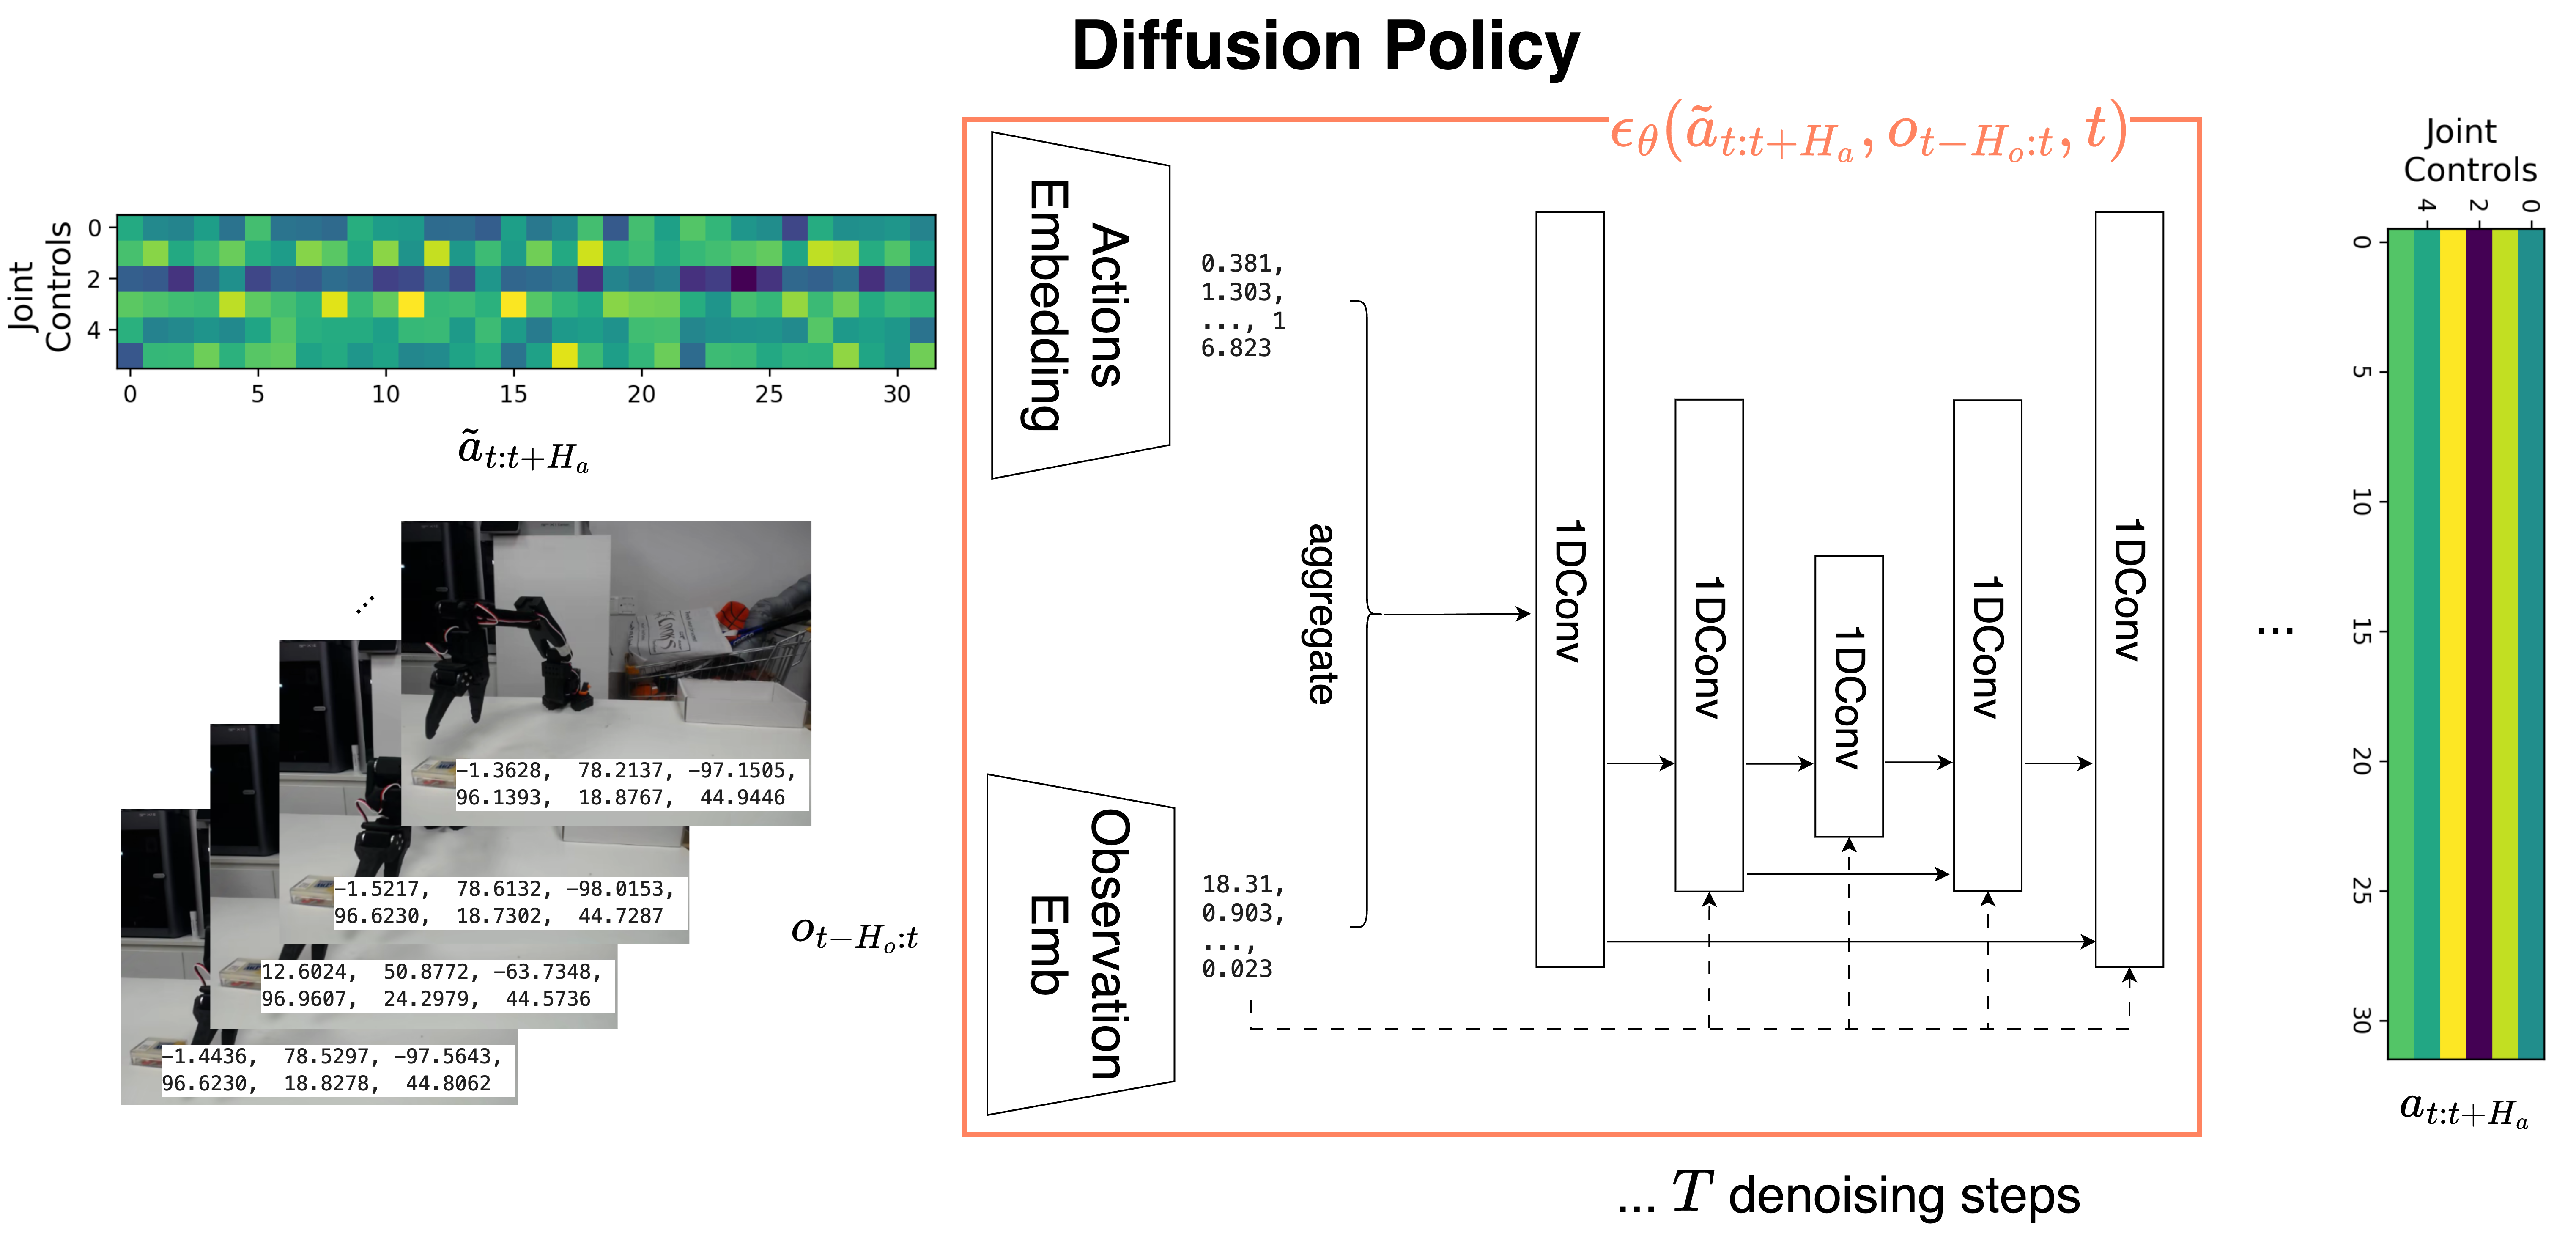
\includegraphics[width=0.9\textwidth]{figures/ch4/ch4-diffusion-policy.png}
    \caption{The Diffusion Policy archicture, as in~\citet{chiDiffusionPolicyVisuomotor2024}. A stack of \( H_o \) previous observations is used as external conditioning to denoise a group of \( H_a \) actions. Conditioning is used at every layer of a U-Net block, and in practice allows to obtain fully-formed action chunks with as little as \(T=10\) denoising steps.}
    \label{fig:diffusion-policy-architecture}
\end{figure}

Figure~\ref{fig:diffusion-policy-architecture} shows the convolution-based version of the architecture proposed by~\citet{chiDiffusionPolicyVisuomotor2024}, illustrating inference on a single sample from \( \mathcal D \) for simplicity.
An arbitrarily noisy chunk of \( H_a \) actions \(\tilde a_{t:t+H_a} \) is mapped to a learned high-dimensional space. 
Similarily, both image observations and poses are embedded before being aggregated to the action embeddings.
Then, a U-Net~\citep{ronnebergerUNetConvolutionalNetworks2015} is trained to regress the noise added into \( \tilde a_{t:t+H_a} \), using observation conditioning information at every layer and seeking to optimize~\ref{eq:diffusion-policy-objective}.
At inference time, the noise predictor is used to predict the quantity of noise at every \( t \in [T, \dots, 0 ] \) and iteratively subtract it from \(\tilde a_{t:t+T_a} \), reversing the diffusion process simulated in training conditioned on \(o_{t-T_o:t} \) to predict \(a_{t:t+T_a} \).

Training using 50-150 demos (15-60 minutes of teleoperation data) DP achieves strong performance on a variety of simulated and real-world tasks, including dexterous and deformable manipulation tasks such as sauce pouring and mat unrolling.
Notably, the authors ablated the relevance of using RGB camera streams as input to their policy, and observed how high frame-rate visual observations can be used to attain performance (measured as success rate) comparable to that of state-based policies, typically trained in simulation with priviledged information not directly available in real-world deployments.
As high-frame rate RGB inputs naturally accomodate for dynamic, fast changing environments,~\citet{chiDiffusionPolicyVisuomotor2024}'s conclusion offers significant evidence for learning streamlined control policies directly from pixels.
In their work,~\citet{chiDiffusionPolicyVisuomotor2024} also ablate the performance of DP against their baseline against the size of the dataset collected, showing that DP outperforms the considered baseline for every benchmark size considered.
Further, to accelerate inference,~\citet{chiDiffusionPolicyVisuomotor2024} employ Denoising Diffusion Implicit Models~\citep{songDenoisingDiffusionImplicit2022}, a variant of Denoising Diffusion Probabilistic Models~\citep{hoDenoisingDiffusionProbabilistic2020} (DDPM) adopting a strictly deterministic denoising paradigm (differently from DDPM's natively stochastic one) inducing the same final distribution's as DDPM's, and yet resulting in 10 times less denoising steps at inference time~\citep{chiDiffusionPolicyVisuomotor2024}.
Across a range of simulated and real-world tasks,~\citet{chiDiffusionPolicyVisuomotor2024} find DPs particularly performant when implementing a transformer-based network as \( \epsilon_\theta \), although the authors note the increased sensitivity of transformer networks to hyperparameters and thus explicitly recommend starting out with a simpler, convolution-based architecture for diffusion (Figure~\ref{fig:diffusion-policy-architecture}), which are however reported to be biased towards learning low-frequency components~\citep{tancikFourierFeaturesLet2020} and thus may prove more challenging to train with non-smooth action sequences.


\subsubsection{Code Example: Learning Diffusion Policies}
\todo{using diffusion policy example}

\subsection{Optimized Inference by Decoupling Action Prediction and Execution}
Modern visuomotor policies output \emph{action chunks}--sequences \(\pi(o_t) = \actionchunk_t \) with \(\actionchunk_t = \bigl(a_t,a_{t+1},\dots,a_{t+H_a}\bigr) \) being a sequence of \(H_a \gg 1 \) low-level commands enqueued in an action queue, originating from an environment observation, \(o_t\).
Predicting series of actions instead of single commands proved essential in learning complex, multi-modal behavior~\citep{zhaoLearningFineGrainedBimanual2023,chiDiffusionPolicyVisuomotor2024}.

Typically, the robot executes the entire action chunk \(\actionchunk_t \), before a new observation \( o_{t+H_a} \) is passed to the policy \( \pi \) to predict the next chunk. 
This results in open-loop inference in between observations captured every \( H_a \) timesteps.
~\citet{zhaoLearningFineGrainedBimanual2023} adopts a different strategy whereby the robot controller interleaves chunk prediction \( \actionchunk_t \gets \pi(o_t) \) and chunk consumption \( a_t \gets \textsc{PopFront(\( \actionchunk_t \))} \), computing a new chunk of actions at every timestep \( t \) and aggregating the predicted chunks on overlapping sections.
While adaptive---every observation at every timestep \( o_t\) is processed---such approaches rely on running inference continuously, which can be prohibitive in resource-constrained scenarios, such as edge deployments.

A less resource-intensive approach is to entirely exhaust the chunk \( \actionchunk \) before predicting a new chunk of actions, a strategy we refer to as \emph{synchronous} (sync) inference. 
Sync inference efficiently allocates computation every \( H_a \) timesteps, resulting in a reduced average computational burden at control time. 
In contrast, it inherently hinders the responsiveness of robot systems, introducing blind lags due to the robot being \emph{idle} while computing \( \actionchunk \).

We directly assess the lack of adaptiveness of robot systems due to acting open-loop, and the presence of lags at runtime by decoupling action chunk prediction \( \actionchunk \) from action execution \( a_t \gets \textsc{PopFront}(\actionchunk_t) \), developing an \emph{asynchronous} (async) inference stack (\ref{alg:async-inference}), whereby a \( \textsc{RobotClient} \) sends an observation \( o_t \) to a \( \textsc{PolicyServer} \), receiving an action chunk \( \actionchunk_t \) once inference is complete (\ref{fig:ch4-async-inference}).
In this, we avoid execution lags by triggering chunk prediction while the control loop is still consuming a previously available queue, aggregating it with the newly incoming queue whenever available.
In turn, async-inference tightens the loop between action prediction and action execution, by increasing the frequency at which observations are processed for chunk prediction.
Crucially, decoupling action prediction from action execution also directly allows to allocate more computational resources on a remote policy server sending actions to the robot client over networks, something which may prove very effective in resource-constrained scenarios such as low-power robots.

\begin{figure}
    \centering
    \begin{minipage}[t]{\textwidth}
        \centering
        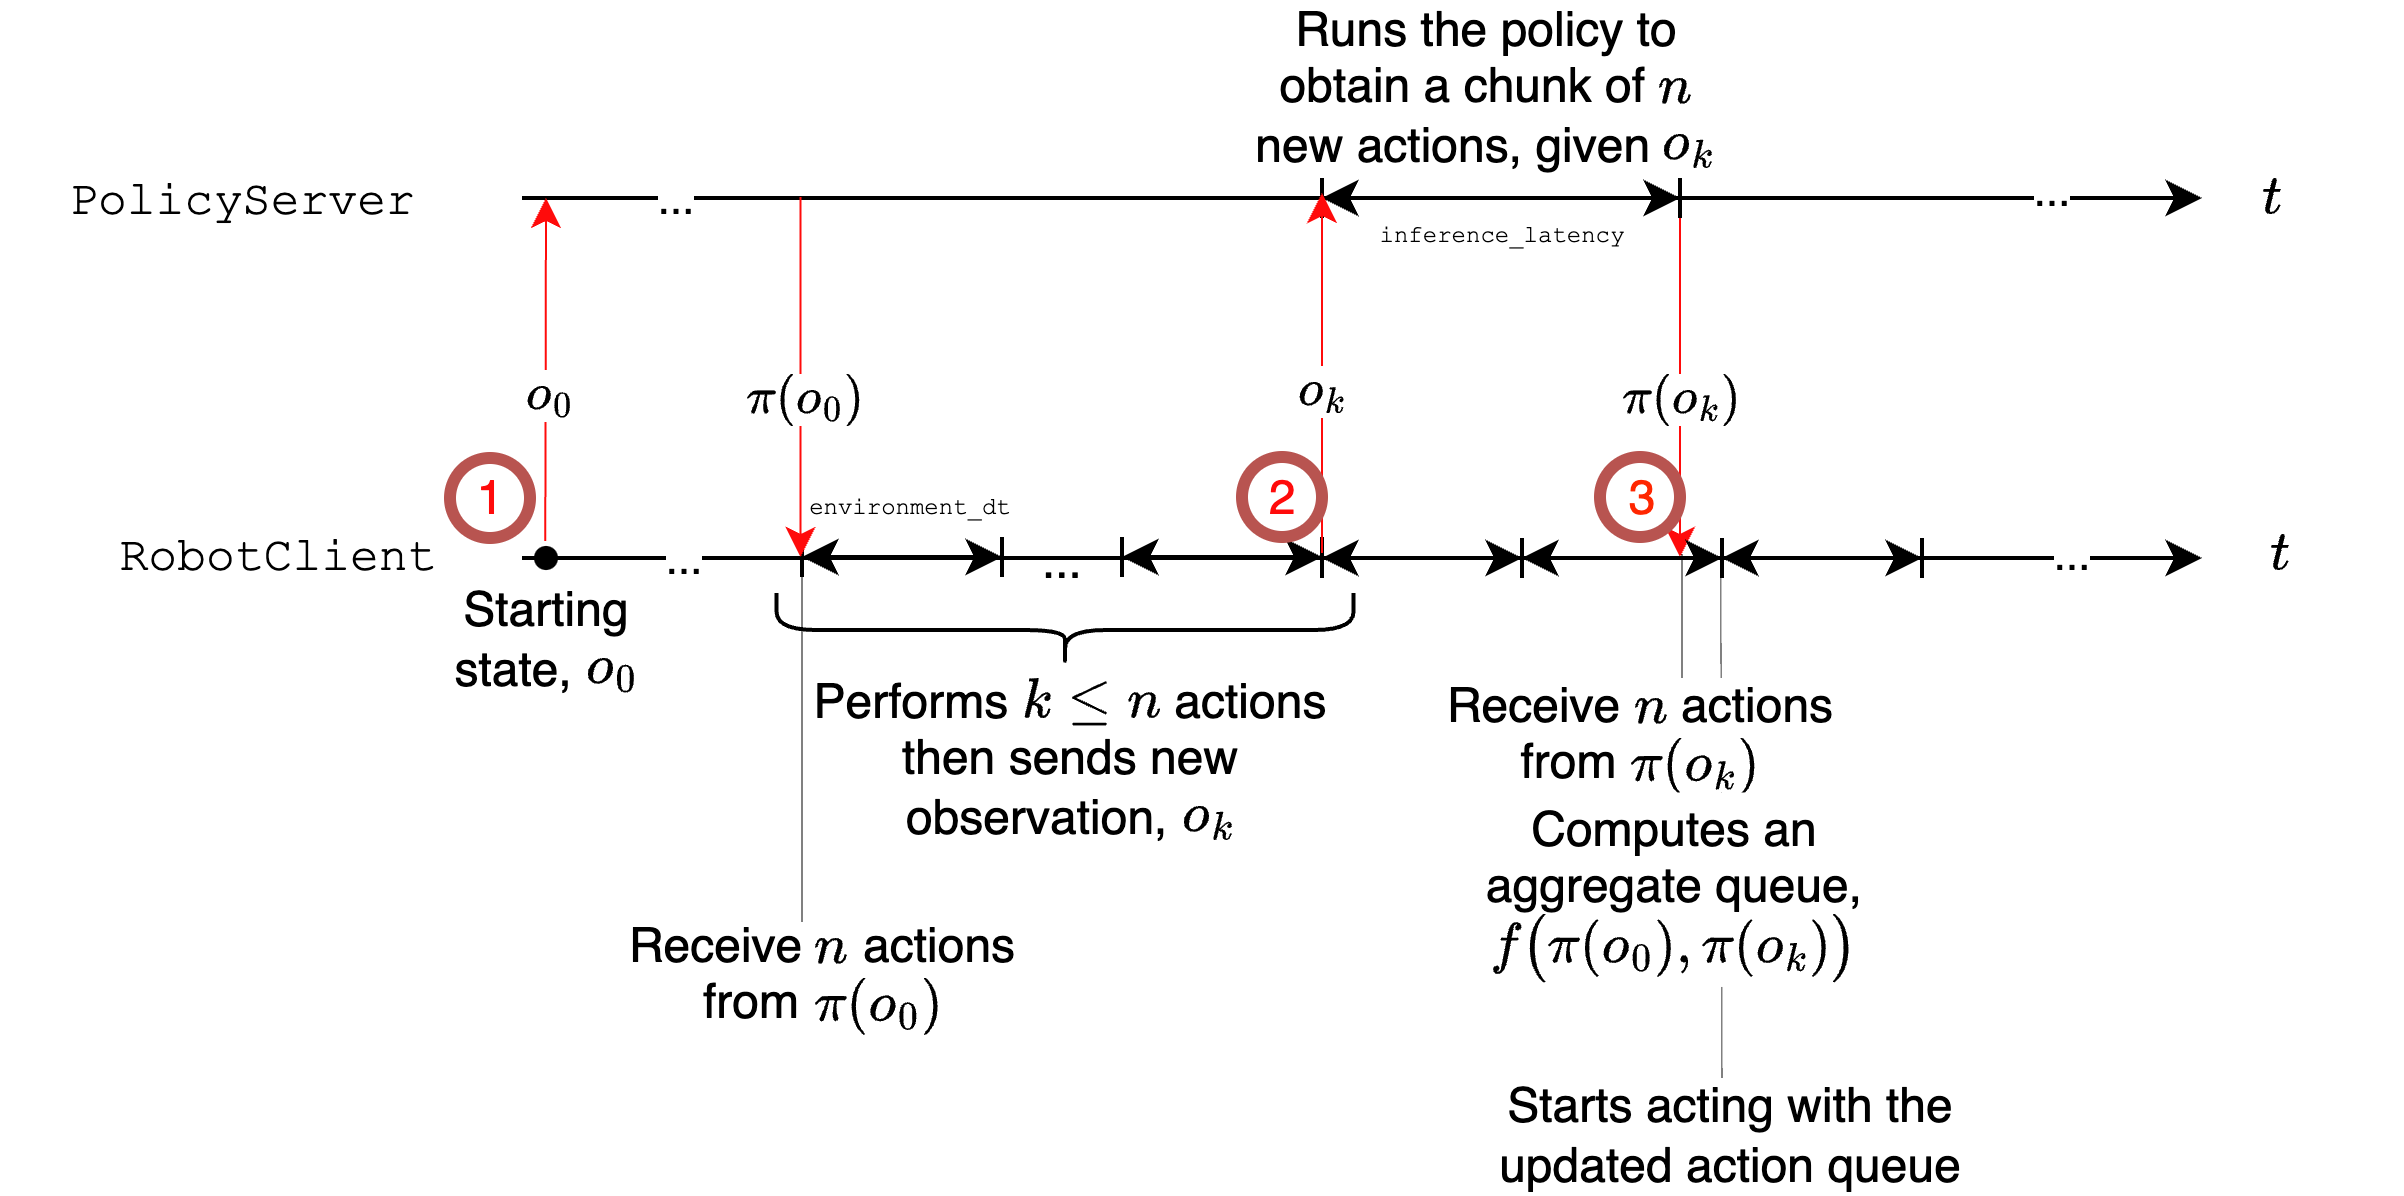
\includegraphics[width=0.9\textwidth]{figures/ch4/ch4-async-inference.png}
        \caption{\textbf{Asynchronous inference}. Illustration of the asynchronous inference stack. Note that the policy can be run on a remote server, possibly with GPUs.}
        \label{fig:ch4-async-inference}
    \end{minipage}
    \vspace{-0.6cm}
\end{figure}

\begin{algorithm}
  \caption{Asynchronous inference control-loop}
  \label{alg:robotclient}
  \begin{algorithmic}[1]
    \State \textbf{Input:} horizon \( T \), chunk size \( H_a \), threshold \( g\in[0,1] \)
    \State \textbf{Init:} capture \( o_0 \); send \( o_0 \) to \textsc{PolicyServer};
           receive \( \actionchunk_0 \gets \pi(o_0) \)
    \For{\( t \) \textbf{to} \( H_a \)}
        \State \( a_t \gets \textsc{PopFront}(\actionchunk_t) \)
        \State \textsc{Execute}(\( a_t \)) \Comment{execute action at step \( t \)}
        \If{\( \tfrac{|\actionchunk_t|}{H_a} < g \)} \Comment{queue below threshold}
            \State capture new observation, \( o_{t+1} \)
            \If{\textsc{NeedsProcessing} \( (o_{t+1}) \) } \Comment{similarity filter, or triggers direct processing}
                \State \texttt{async\_handle} \( \gets \textsc{AsyncInfer}(o_{t+1})\) 
                \Comment{Trigger new chunk prediction (non blocking)}
                \State \( \tilde{\actionchunk}_{t+1} \gets \pi(o_{t+1}) \) \Comment{New queue is predicted with the policy}
                \State \( \actionchunk_{t+1} \gets f(\actionchunk_t,\tilde{\actionchunk}_{t+1}) \) \Comment{aggregate overlaps (if any)}
                
            \EndIf
        \EndIf
        \If {\textsc{NotCompleted}(\texttt{async\_handle})}
            \State \( \actionchunk_{t+1} \gets \actionchunk_t \) \Comment{No update on queue (inference is not over just yet)}
        \EndIf
    \EndFor
  \end{algorithmic}
  \label{alg:async-inference}
\end{algorithm}


\paragraph{Implementation details}

\emph{Async} inference (1) tightens the control loop by capturing observations more often, directly eliminates idle gaps at runtime, and (2) directly allows to run inference on more powerful computational resources than the ones typically available onboard autonomous robotic platforms.

Algorithmically, we attain (1) on the \textsc{RobotClient}-side by consuming actions from a readily available queue until a threshold condition on the number of remaining actions in the queue (\(\vert \actionchunk_t \vert / H_a < g \)) is met. When this condition is triggered, a new observation of the environment is captured and sent to the (possibly remote) \textsc{PolicyServer}. 
To avoid redundant server calls and erratic behavior at runtime observations are compared in joint-space, and near-duplicates are dropped.
Two observations are considered near-duplicates if their distance in joint-space is under a predetermined threshold, \( \epsilon \in \mathbb R_+\).
Importantly, when the queue available to robot client eventually becomes empty, the most recent observation is processed regardless of similarity.

Interestingly, the behavior of async inference can be studied analytically. First, let \( \ell \) be a random variable modeling the time needed to receive an action chunk \( \actionchunk \) after sending an observation \( o \), i.e. the sum of (1) the time to send across the observation \( o \) between the \textsc{RobotClient} and \textsc{PolicyServer}, \( t_{C \to S}\) (2) the inference latency on the \textsc{PolicyServer}, \( \ell_S \) and (3) the time to send \( \actionchunk \) between the \textsc{PolicyServer} and \textsc{RobotClient}, \( t_{S \to C} \). Assuming independence, \( \mathbb E [\ell] = \mathbb E[t_{C \to S}] + \mathbb E[\ell_S] + \mathbb E[t_{S \to C}] \) which can be further simplified to \( \mathbb E[\ell] \simeq \mathbb E[\ell_S]  \), assuming communication time is (1) equal in both directions and (2) negligible with respect to the inference latency. Second, let \(\Delta t\) be the environment’s control cycle. With a real-world frame-rate of 30 frames per second, \(\Delta t=33\text{ms}\). Consequently, exhausted queues at runtime--i.e. being idle awaiting for a new chunk--are avoided for \( g \geq \frac{\mathbb E[\ell_S] / \Delta t}{H_a} \). In this, the queue threshold \( g \) plays a major role relatively to the availability of actions to the \textsc{RobotClient}.

\ref{fig:ch4-queues} illustrates how the size of the action chunk \(\lvert \actionchunk_t \rvert\) evolves over time for three representative values of \(g\), detailing the following key scenarios:
\begin{itemize}
    \item \textbf{Sequential limit \((g=0)\).} The client drains the entire chunk before forwarding a new observation to the server. During the round-trip latency needed to compute the next chunk, the queue is empty, leaving the robot \emph{incapable of acting}.  This reproduces the behavior of a fully sequential deployment and results in an average of \( \mathbb E[\ell_S] \) idle seconds.
    \item \textbf{Asynchronous inference \((g \in (0,1))\).} Allowing the client to consume \(1-g\) of its available queue \( \actionchunk_{t-1}\) before triggering inference for a new action queue \( \actionchunk_{t} \), amortizing computation while keeping the queue from emptying. The overlap between successive chunks provides a buffer against modeling errors without the full cost of the \(g=1\) regime. The updated queue \( \actionchunk_t\) is obtained aggregating queues on the overlapping timesteps between \( \actionchunk_{t-1}\) and the incoming \(\tilde{\actionchunk}_{t}\).
    \item \textbf{Compute-intensive limit \((g=1)\).}  As an extreme case, and in keeping with \citet{zhaoLearningFineGrainedBimanual2023}, an observation is sent at \emph{every} timestep. The queue is therefore almost always filled, with only a minor saw-tooth due to \(\Delta t/\mathbb E[\ell_s] < 1\). While maximally reactive, this setting incurs one forward pass per control tick and can prove prohibitively expensive on limited hardware. Importantly, because the client is consuming actions while the server computes the next chunk, the available queue never gets filled again.
\end{itemize}

\begin{figure}
    \centering
    \begin{minipage}[t]{0.99\textwidth}
        \centering
        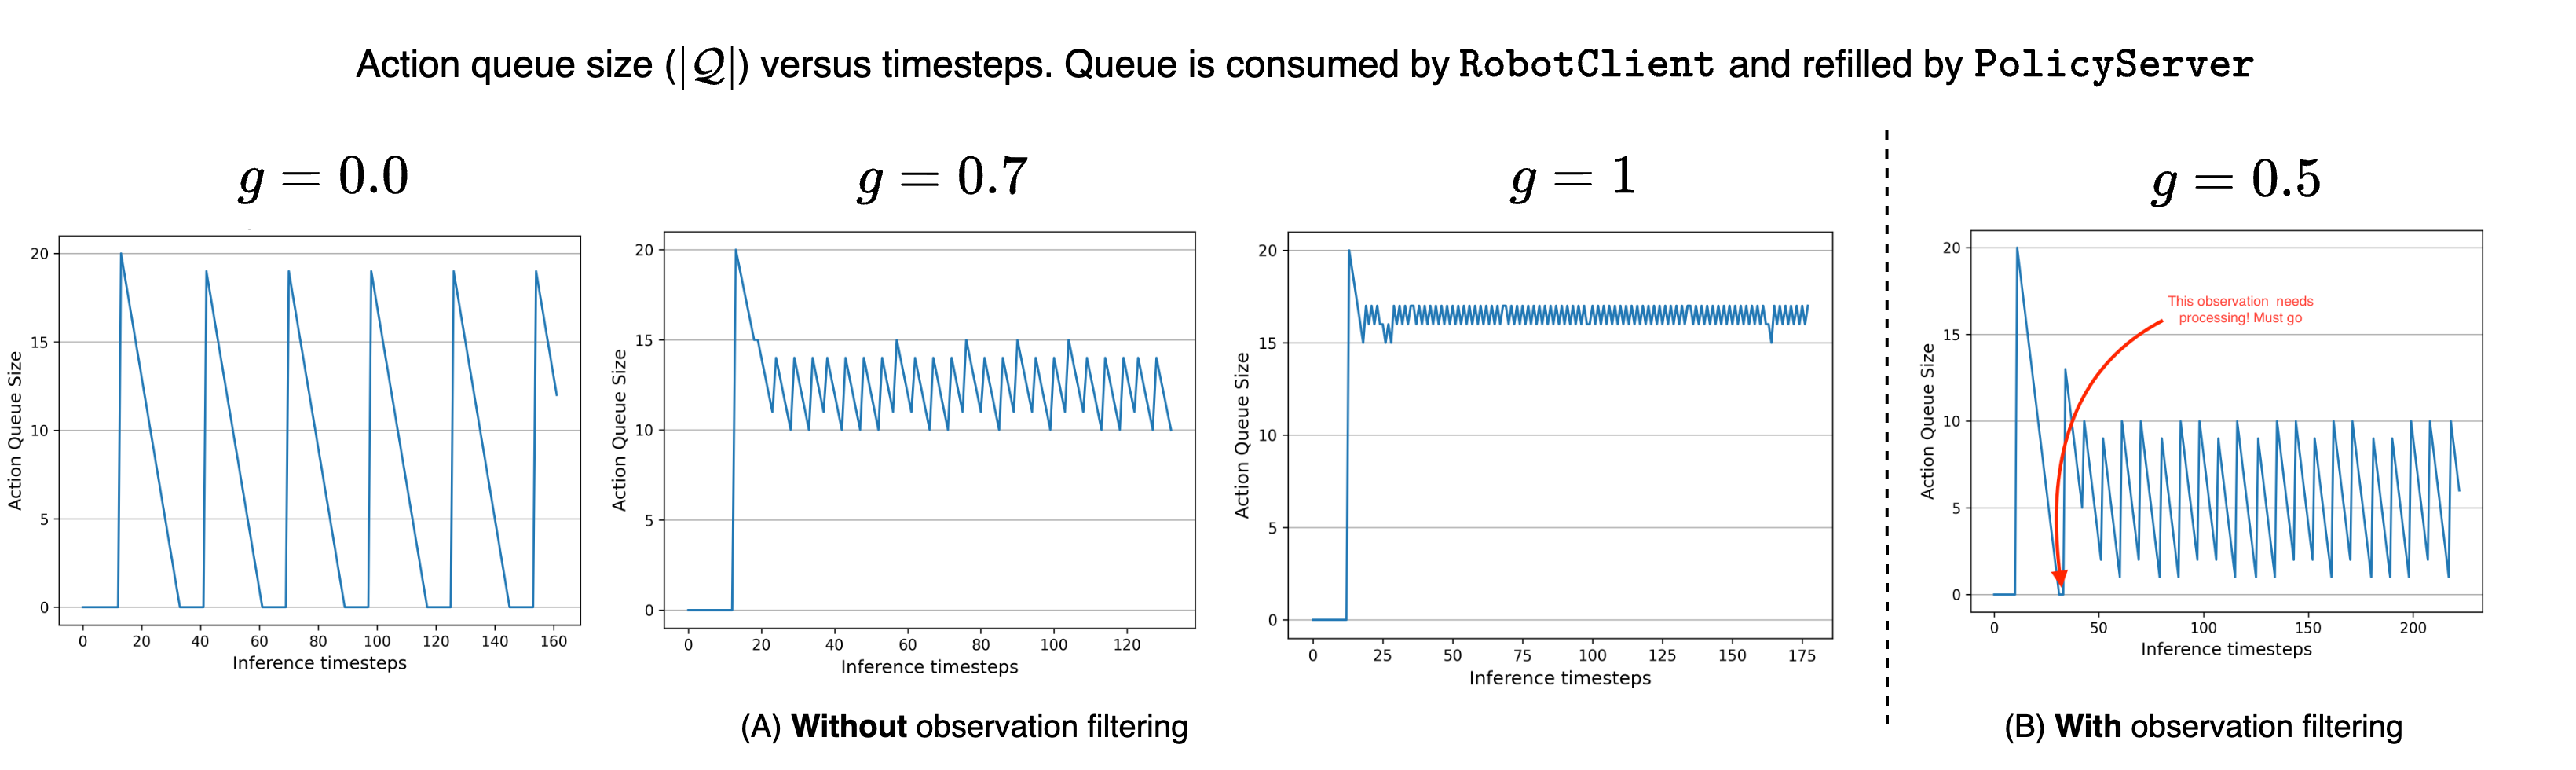
\includegraphics[width=\textwidth]{figures/ch4/ch4-queues.png}
        \caption{Action queue size evolution at runtime for various levels of \( g\) when (A) not filtering out observation based on joint-space similarity and (B) filtering out near-duplicates observation, measuring their similarity in joint-space.}
        \label{fig:ch4-queues}
    \end{minipage}
\end{figure}

\ref{fig:ch4-queues} emphasizes the trade-off governed by \(g\): small values place result in idle periods, whereas \(g\approx 1\) assumes a highly accurate model and pays a significant compute price. In practice, choosing \(g\in(0,1)\) allows to strike a balance between reactivity against resource budgets. 
If not for the aforementioned similarity filter, the \textsc{RobotClient} would send observations for processing every \( (1 - g) H_a \cdot \Delta t\) seconds, receiving a new chunk of actions every \( (1 - g) H_a \cdot \Delta t + \mathbb E[\ell_S] \), on average. 
The presence of the observation similarity filter dilates this processing time, and serves the scope of avoiding the robot stalling due to the queue being constantly integrated with an incoming, nearly identical, action chunk. 
In particular,~\ref{fig:ch4-queues} results in a queue which is filled with incoming actions \emph{unless} near-duplicate observations are filtered out from the processing pipeline. For clarity, the red arrow in~\ref{fig:ch4-queues} highlights a timestep where the observation similarity mechanism is bypassed, forcing a (nearly identical) observation to be processed as the queue results empty.

\subsubsection{Code Example: Using Async Inference}
\todo{async inference example}